%\motto{Use the template \emph{chapter.tex} to style the various elements of your chapter content.}
\chapter{Quanteninformationen}
\label{qbits} % Always give a unique label
% use \chaptermark{}
% to alter or adjust the chapter heading in the running head

\chapterauthor{Dominik Neumaier, Hannes Ringswald, Marvin Rothmann, Thilo Prünte}

\abstract{}
Dieses Kapitel führt in die Grundlagen der Quanteninformation ein. Es erläutert die Unterschiede zwischen klassischen Bits und Qubits, beschreibt zentrale Konzepte wie Superposition, Verschränkung und Quantenparallelismus und stellt grundlegende Quanten-Gatter vor. Anhand der Algorithmen von Deutsch und Deutsch-Josza wird das Potenzial quantenmechanischer Berechnungen demonstriert. Zudem behandelt das Kapitel die Prinzipien der Quantenteleportation, Quantenkommunikation sowie die Bedeutung von Bell-Zuständen und Quantenfehlerkorrektur. Damit bietet es einen Überblick über die theoretischen Grundlagen und ersten Anwendungen der Quanteninformation.

\section{Das Qubit als Informationsträger}
\label{Das Qubit als Informationsträger}
\subsection{Klassisches Bit vs.\ Qubit}
Ein \emph{Bit} ist die kleinste Informationseinheit in klassischen Computern. Es kann genau einen von zwei Zuständen annehmen: $\text{Bit}\,\in\{0,1\}$.
Physikalisch bedeutet das zum Beispiel: Strom an = 1, Strom aus = 0. Durch Schaltkreise, die verschiedene logische Operatoren abbilden, können so Berechnungen durchgeführt werden oder durch spezielle Kodierungen (zum Beispiel ASCII) Daten repräsentiert werden.

In \emph{Quantencomputern} werden analog dazu \emph{Qubits} (Quantenbits) als grundlegende Informationseinheiten verwendet. Ein Qubit wird hier als abstraktes mathematisches Objekt behandelt, dessen Konzept auf alle konkreten physikalischen Implementierungen anwendbar ist, die im späteren Teil dieses Buches erläutert werden.

Wie ein klassisches Bit hat auch ein Qubit zwei mögliche Zustände: $\ket{0}$ und $\ket{1}$. Die Notation, die zur Beschreibung verwendet wird, heißt \emph{Bra-Ket-Notation}. Der entscheidende Unterschied zu einem konventionellen Bit ist, dass ein Qubit auch andere Zustände als $\ket{0}$ und $\ket{1}$ annehmen kann. Konkret kann es eine lineare Kombination der beiden Zustände, eine sogenannte Superposition (vgl. Kapitel irgendwas in physikalische Grundlagen), einnehmen. Dies wird folgendermaßen beschrieben:
\begin{equation}
    \ket{\psi} = \alpha\,\ket{0} \;+\; \beta\,\ket{1}, \quad \alpha, \beta \in \mathbb{C},
\end{equation}
wobei die Koeffizienten \(\alpha\) und \(\beta\) komplexe Zahlen sind, die als \emph{Amplituden} bezeichnet werden. Der Zustand eines Qubits liegt also in einem komplexen Raum.

Für die Amplituden \(\alpha\) und \(\beta\) gilt:
\begin{equation}
\label{equ:propa}
|\alpha|^2 + |\beta|^2 = 1.
\end{equation}
Die Betragsquadrate \(|\alpha|^2\) und \(|\beta|^2\) repräsentieren die Wahrscheinlichkeiten, das Qubit bei einer Messung in den Zuständen \(\ket{0}\) beziehungsweise \(\ket{1}\) zu finden. Die Normierungsbedingung \ref{equ:propa} gewährleistet, dass die Gesamtwahrscheinlichkeit für alle möglichen Messergebnisse eins beträgt, was der fundamentalen Anforderung der Wahrscheinlichkeitstheorie entspricht.

Die komplexe Natur der Amplituden ermöglicht es, dass Qubits nicht nur klassische Überlagerungen von Zuständen darstellen, sondern auch komplexe Phasenbeziehungen zwischen den Basiszuständen kodieren können. Diese Eigenschaft bildet die Grundlage für die charakteristischen Quanteneffekte, die Quantencomputer von klassischen Computern unterscheiden. (vgl. \cite[13 ff.]{nielsen_quantum_2010}, \cite[13 ff.]{rieffel_quantum_2011}, \cite{matuschak_quantum_2019})

Als Beispiel soll hier folgender Qubit-Zustand dienen, welcher im Verlauf des Buches häufiger als Beispiel verwendet wird:
\begin{equation}
\label{equ:basicZustand}
    \frac{1}{\sqrt{2}}\ket{0} + \frac{1}{\sqrt{2}}\ket{1}
\end{equation}
Um zu überprüfen, ob dies ein gültiger Qubit-Zustand ist, werden die Werte in Formel \ref{equ:propa} eingesetzt:
\begin{equation}
    \left|\frac{1}{\sqrt{2}}\right|^2 + \left|\frac{1}{\sqrt{2}}\right|^2 = 0{,}5 + 0{,}5 = 1
\end{equation}
Damit ist gezeigt, dass die Normierungsbedingung erfüllt ist und die Wahrscheinlichkeit, einen der beiden Zustände zu messen, jeweils $0{,}5$ beträgt.
Wie diese Beschreibung zeigt, kann ein einzelnes Qubit nach einer Messung zunächst auch nur zwei Zustände repräsentieren und ist damit als einzelnes nicht mächtiger als ein einzelnes Bit. Die Stärke von Qubits wird dann sichtbar, wenn mehrere kombiniert werden (siehe Kapitel \ref{subsec:verschraenkungQubits}). (vgl. \cite[14]{nielsen_quantum_2010})

\subsection{Bloch-Kugel}\label{subsec:blockkugel}
Ein Qubit-Zustand lässt sich dreidimensional in einer anschaulichen Art darstellen: Als Punkt auf der Einheitssphäre $ \mathbb{R}^ 3 $. Dabei wird von einer \emph{Bloch-Kugel} gesprochen. Jeder Zustand
kann durch zwei Winkel $\phi$ und $\theta$ beschrieben werden:

\begin{figure}[H]
  \centering
  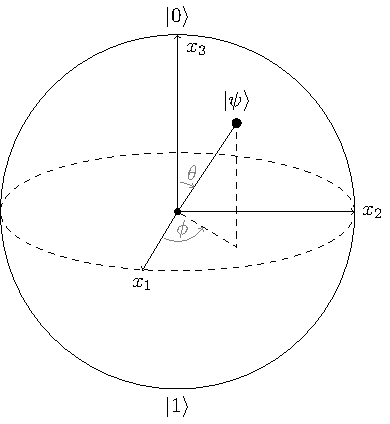
\includegraphics[width=0.7\textwidth]{images/quantum-information/bloch.pdf}
  \caption{Bloch-Kugel (Darstellung angelehnt an \cite{riebesell_scientific_2022})}\label{fig:bloch-sphere}
\end{figure}

Der Zustand des Qubits kann folgendermaßen berechnet werden:

\begin{equation}
  \ket{\psi} = \cos\frac{\theta}{2} \ket{0} + e^{i\phi} \sin\frac{\theta}{2} \ket{1}
\end{equation}

Ein Qubit kann also eine unendliche Anzahl an Zuständen annehmen. Das ließe die Vermutung zu, dass ein Qubit auch unendlich viele Informationen speichern kann. Dies ist jedoch nicht der Fall, weil beim Messen des Zustandes die Superposition zusammenfällt und das Qubit dann entweder den Wert $\ket{0}$ oder $\ket{1}$ hat. (vgl. [5 ff.]\cite{pattanayakQuantumMachineLearning2017}, \cite[15 f.]{nielsen_quantum_2010}

\subsection{Informationscodierung}
Eine zentrale Herausforderung im Quantencomputing ist die effiziente Codierung klassischer Daten in Quantenzustände. Quantenalgorithmen operieren auf Zuständen, die in einem Hilbertraum beschrieben werden – nicht auf klassischen Bitmustern. Um Daten quantenmechanisch verarbeiten zu können, müssen sie daher in geeignete Qubitzustände übersetzt werden.

Je nach Art der Daten und Anforderungen des Algorithmus existieren unterschiedliche Codierungsmethoden. Diese unterscheiden sich unter anderem in der Anzahl benötigter Qubits, in ihrer Fähigkeit zur Darstellung kontinuierlicher oder diskreter Werte, sowie im Aufwand zur Zustandspräparation und -messung. Dieses Kapitel stellt die wichtigsten Codierungstechniken vor.

\subsubsection{Basis-Encoding}
\begin{itemize}
\item Ziel: Direkte Abbildung binärer klassischer Daten auf die Computational-Basiszustände von Qubits
\item Jeder Datenwert wird 1:1 als Bitstring interpretiert und im Quantenregister als entsprechender Basiszustand gespeichert
\item Es entsteht keine Superposition – jeder Qubit-Zustand steht für genau einen Datenwert
\item Grundlage vieler Quantenalgorithmen mit diskreten Datenstrukturen (z.\,B. Suchalgorithmen, Entscheidungsprobleme)
\item Daten sind binär codiert (z.\,B. $ x_1 = 101, x_2 = 011$)
\item Jeder Datenwert = ein spezifischer Basiszustand im Quantenregister (z.\,B. $\ket{101}$)
\item Auch geschrieben als $\ket{101} = \alpha\ket{1} \otimes \beta \ket{0} \otimes \gamma\ket{1}$ wobei das Tensorprodukt $\otimes$ darstellt, dass die Qubits unabhängig voneinander zu sehen sind
\item Für \( n \) Bit lange Daten: benötigt werden $n$ Qubits
\end{itemize}
\cite{Date encoding patterns for quantum computing}
\\

Anwendungsbeispiel 1
\begin{itemize}
\item Gegeben: Zwei Werte $x_1 = 101$, $x_2 = 011$
\item Jeder Wert ist 3 Bit lang → 3 Qubits nötig
\item Quantenregister speichert z.\,B. einzeln $\ket{101}$ oder $ \ket{011}$
\item Darstellung 
\item Keine Superposition oder Interferenz enthalten – Datenzugriff erfolgt deterministisch (wenn exakt vorbereitet)
\item Nach Messung: genau der gespeicherte Basiszustand wird gelesen (sofern keine Quantenoperationen dazwischentreten)
\end{itemize}

Anwendungsbeispiel 2 – Text „hello“
\begin{itemize}
\item ASCII-Codierung von „hello“:
\begin{itemize}
    \item $\ket{h} = \ket{1101000}$
    \item $\ket{e} = \ket{1100101}$
    \item $\ket{l_1} = \ket{1101100}$
    \item $\ket{l_2} = \ket{1101100}$
    \item $\ket{o} = \ket{1101111}$
    
\end{itemize}
\item Darstellung: „hello“ → Folge von fünf 8-Bit-Binärwerten
\item Gesamtanzahl benötigter Qubits: $5 \times 8 = 40$
\item Quantenregister speichert z.\,B. $\ket{1101000\,1100101\,1101100\,1101100\,1101111}$
\item Nach Messung: exakt dieser Bitstring wird gelesen (sofern Zustand nicht verändert wurde)
\item Wichtig: Keine Quantenparallelität in dieser Form – rein klassisch gespeicherte Information auf einem Quantenregister
\end{itemize}
\cite{Quantum Data Encoding: A Comparative Analysis of Classical-to-Quantum Mapping Techniques and Their Impact on Machine Learning Accuracy}


\subsubsection{QuAM Encoding}
\begin{itemize}
\item Ziel: Sammlung mehrerer Datenwerte und Speicherung im Quantenregister (Sammlung mehrerer Qubits, die gemeinsam einen Zustand beschreiben)
\item Quantenalgorithmus benötigt mehrere Zahlenwerte \( x_1, x_2, \ldots \) als Input
\item Daten in einem gemeinsamen Qubit-Register als Superposition von Basis-encodierten Zuständen speichern
\item Ergebnis: Gleichgewichtete Superposition aller Datenwerte mit Amplituden (hohe Wahrscheinlichkeiten gemessen zu werden)
\item Daten sind binär codiert (z.\,B. \( x_1 = 010, x_2 = 011, x_3 = 110 \))
\item Jeder Datenwert = ein Basiszustand im Quantenregister (z.\,B. \( |010\rangle \))
\item Für \( n \) Werte mit je \( l \) Bit: benötigt werden \( l \) Qubits
\end{itemize}
\cite{Date encoding patterns for quantum computing}
\\


Anwendungsbeispiel
\begin{itemize}
\item Gegeben: Drei Werte \( x_1 = 010 \), \( x_2 = 011 \), \( x_3 = 110 \)
\item Jeder Wert ist 3 Bit lang → 3 Qubits nötig
\item Quantenregister speichert:
  \[
  |\psi\rangle = \frac{1}{\sqrt{3}} (|010\rangle + |011\rangle + |110\rangle)
  \]
\item Nur diese drei Zustände haben Amplituden, alle anderen (z.\,B. \( |000\rangle, |001\rangle \)) = 0
\item Nach Messung: Einer der gespeicherten Werte wird mit Wahrscheinlichkeit \( \frac{1}{3} \) gelesen
\end{itemize}

\subsubsection{Angle Encoding}

\begin{itemize}
\item Jeder Datenpunkt wird durch ein separates Qubit repräsentiert.
\item Ziel: Daten effizient auf einem Quantencomputer kodieren, um möglichst viele Operationen innerhalb der Stabilitätsdauer des Quantenzustands durchzuführen.
\item Jeder Wert \(x_i\) wird auf das Intervall \([0, \frac{\pi}{2}]\) normalisiert.
\item Bereich \([0, \frac{\pi}{2}]\), weil \(\cos(x)\) und \(\sin(x)\) dort positiv sind → keine Vorzeichenprobleme
\item Ein einzelnes Qubit repräsentiert einen Datenwert durch  Rotation um die y-Achse auf der Bloch-Kugel.
\item Die resultierende Quantenzustand ist separabel, d.h. es findet keine Verschränkung der Qubits statt.
\item Der Zustand ergibt sich als Tensorprodukt einzelner Qubit-Zustände: 
\[
|\psi\rangle = \bigotimes_i \begin{bmatrix} \cos x_i \\ \sin x_i \end{bmatrix}
\]
\item Vorteil: Sehr effizient in Bezug auf Operationen – konstante Anzahl paralleler Einzelqubit-Rotationen genügt.
\item Nachteil: Für \(n\) Datenwerte werden \(n\) Qubits benötigt – nicht optimal im Qubit-Bedarf.
\item Anwendungen: Klassifikatoren, Quantum Image Processing (ein Qubit = Farbwert, Register = Position), Quantum Neural Networks (Quron).
\end{itemize}
\cite{encoding patterns for quantum algorithms}
\\


Anwendungsbeispiel:
\begin{itemize}
\item \textbf{Beispiel:} Temperaturen in Städten speichern – Berlin: 15°C, Paris: 25°C, Madrid: 30°C
\item \textbf{Schritt 1:} Normalisieren auf Bereich \([0, \frac{\pi}{2}]\)
  \begin{itemize}
    \item 15°C → 45°, 25°C → 75°, 30°C → 90°
  \end{itemize}
\item \textbf{Schritt 2:} Visualisierung: Jede Temperatur entspricht einem Zeiger (Qubit) auf einer Uhr
\item \textbf{Schritt 3:} Zeiger wird um Winkel gedreht (z.\,B. 45°)
\item \textbf{Schritt 4:} Drehung entspricht Rotation eines Qubits um y-Achse
\item \textbf{Schritt 5:} Jeder Qubit-Zustand speichert seinen Drehwinkel
\item \textbf{Schritt 6:} Kombination aller Qubits = Gesamtzustand des Systems
\end{itemize}


\subsubsection{QRAM Encoding}

\begin{itemize}
    \item Quantum Random Access Memory Encoding
    \item Wie im klassischen RAM wird eine Adresse mit einem Speicherindex übergeben. Die Daten an dem Index werden in ein Ausgaberegister geschrieben.
    \item QRAM bietet die gleiche Funktionalität. Die Adresse und das Ausgaberegister sind aber Quantenregister
    \item Die Adresse und das Ausgaberegister können Superposition über mehrere Werte sein
    \item Das Adressregister benötigt $\log(n)$ zusätzliche QBits für $n$ Adressen
    \item Die Daten werden mit Hilfe von Basis-Encoding Codiert
    \item Die Recheneigenschaften sind ähnlich wie die von Basis- oder QuAM-Encoding. Es kann Quantenparallelismus und arithmetische Operationen verwendet werden.
    \item Daten müssen in logarithmischer Laufzeit vorbereitet werden
\end{itemize}

\subsubsection{Amplituden Encoding}
\begin{itemize}
    \item Daten werden in die Amplitude eines Quantenzustands codiert
    \item Es werden $\log(NM)$ QBits benötigt um $M$ Datenpunkte mit $N$ zuständen zu repräsentieren.
\end{itemize}
\begin{itemize}
    \item Wir wollen folgenden Vektor codieren 
    $$
        x = (0.1, -0.7, 1)
    $$
    \item Die Datenpunkte werden Normalisiert und die länge des Vektors auf $2^n$ Datenpunkte angepasst. Hinzugefügt Datenpunkte werden mit $0$ initialisiert. (Hier gerundet auf 3 Nachkommastellen)
    $$
        x = (0.081, -0.571, 0.816, 0.000)
    $$
    \item Der Vektor kann nun mit 2 QBits repräsentiert werden
    $$
          \begin{aligned}
            &0.081|00\rangle \\
            &-0.571|01\rangle \\
            &+0.816|10\rangle \\
            &+0.000|11\rangle
        \end{aligned}
    $$
\end{itemize}

\subsection{Verschränkung von Qubits}
\label{subsec:verschraenkungQubits}

Der eigentliche Nutzen von Qubits zeigt sich dann, wenn mehrere Qubits miteinander kombiniert werden. Während ein einzelnes Qubit sich in einer Überlagerung der Zustände \(0\) und \(1\) befinden kann, erweitert sich der gesamte Zustandsraum beim Hinzufügen weiterer Qubits \emph{exponentiell}.

In klassischen Computern führen \(n\) Bits zu \(2^n\) möglichen Kombinationen von festen Zuständen, wobei sich zu jedem Zeitpunkt aber immer nur \emph{eine} dieser Kombinationen im Arbeitsspeicher befindet. Ein klassisches 3-Bit-System kann zum Beispiel genau einen von acht Zuständen darstellen und gleichzeitig verarbeiten: \(000\), \(001\), ..., \(111\).

Ein Quantensystem aus \(n\) Qubits hingegen befindet sich in einer Superposition all dieser Zustände gleichzeitig. Es existieren also \(2^n\) sogenannte \emph{Basiszustände}, die gleichzeitig in der Beschreibung des Gesamtzustands mit bestimmten Gewichtungen (Wahrscheinlichkeitsamplituden) vorkommen. Der Gesamtzustand eines Qubit-Systems mit \(n\) Qubits kann somit als Superposition aller \(2^n\) möglichen klassischen Kombinationen dargestellt werden.

Jeder dieser Zustände kann gleichzeitig im Gesamtzustand des Systems enthalten sein – mit je einer komplexen Amplitude. Dies bedeutet nicht, dass der Quantencomputer alle Lösungen gleichzeitig kennt, aber dass er während der Berechnung in gewisser Weise mit vielen Möglichkeiten \emph{parallel} arbeiten kann. Dies ist ein einfacher Grund, warum manche Algorithmen auf Quantencomputern eine exponentielle Beschleunigung ermöglichen.

Je mehr Qubits man miteinander verschaltet, desto größer wird also der Zustandsraum. Schon mit wenigen Qubits lassen sich gewaltige Mengen an Zuständen darstellen und zum selben Zeitpunkt verarbeiten: Bei einem Qubit zwei Zustände, bei fünf 32, bei 50 \(\approx 1{,}13 \times 10^{15}\), \dots
An dieser Stelle soll zur Einordnung erwähnt werden, dass der Ende 2023 größte Quantencomputer 433 Qubits hat, das Unternehmen IBM aktuell jedoch einen Quantencomputer mit einer Anzahl von 100 000 Qubits plant.

Das verdeutlicht den fundamentalen Unterschied zwischen Quantencomputern und klassischen Computern in Bezug auf die Informationsverarbeitung. Ein Quantensystem mit $n$ Qubits operiert in einem $2^n$-dimensionalen komplexen Raum, wodurch es theoretisch alle $2^n$ Basiszustände gleichzeitig in einer Superposition verarbeiten kann. Wie eben aufgeführt wären dies für 50 Qubits \(\approx 1{,}13 \times 10^{15}\) (also über eine Billiarde) simultane Berechnungspfade. Bei einem klassischen Computer mit 50 Bits kann nur ein einziger Zustand zu jeder Zeit repräsentiert werden, weshalb diese Anzahl an Berechnungspfaden sequenziell abgearbeitet werden müsste.

Der mathematische Ausdruck für einen allgemeinen $n$-Qubit-Zustand lautet:
\begin{equation}
\ket{\psi} = \sum_{i=0}^{2^n-1} \alpha_i \ket{i}
\label{equ:n_qubit_zustand}
\end{equation}
wobei $\ket{i}$ die Basiszustände und $\alpha_i$ die komplexen Amplituden darstellen. Diese Superposition aller möglichen Basiszustände bildet die Grundlage für die exponentiell gesteigerte Verarbeitungskapazität von Quantencomputern gegenüber klassischen Systemen.

An dieser Stelle soll dargestellt werden, was das für ein 2-Qubit-System mit $n = 2$, also 4 Basiszuständen heißt. Die allgemeine Formel \ref{equ:n_qubit_zustand}
wird zu:
\begin{equation}
\ket{\psi} = \sum_{i=0}^{3} \alpha_i \ket{i} = \alpha_0 \ket{0} + \alpha_1 \ket{1} + \alpha_2 \ket{2} + \alpha_3 \ket{3}
\end{equation}

Die Basiszustände $\ket{0}$, $\ket{1}$, $\ket{2}$, $\ket{3}$ entsprechen den binären Darstellungen $\ket{00}$, $\ket{01}$, $\ket{10}$, $\ket{11}$. Daher lautet die explizite Darstellung:
\begin{equation}
\ket{\psi} = \alpha_0 \ket{00} + \alpha_1 \ket{01} + \alpha_2 \ket{10} + \alpha_3 \ket{11}
\end{equation}

Es ist wichtig zu beachten, dass diese theoretische Parallelität in der praktischen Anwendung durch die Eigenschaften der Quantenmessung und Dekohärenz begrenzt wird, dennoch stellt sie das fundamentale Prinzip dar, das Quantenalgorithmen ihre charakteristische Effizienz verleiht.

Diese enorme Zustandsvielfalt ist nicht einfach direkt auslesbar – bei einer Messung kollabiert das Qubit-System zu genau einem dieser \(2^n\) Basiszustände. Dennoch erlaubt die gleichzeitige Verarbeitung dieser vielen Möglichkeiten innerhalb eines Algorithmus ein grundsätzlich neues Rechenparadigma. Probleme, deren Rechenzeit auf konventionellen Computern exponentiell wächst können deshalb von Quantencomputern in angemessenen Zeiten gelöst werden. 

Es ist sehr wichtig Quantenparallelismus nicht mit dem parallelen Ausführen von Programmen in klassischen Computern gleichzusetzen. Quantenparallelismus nutzt die fundamentalen Eigenschaften der Quantenmechanik, insbesondere die Superposition und die Interferenz von Wahrscheinlichkeitsamplituden. Das heißt, dass es bei Quantenalgorithmen darum geht die Amplituden der Zustände so zu manipulieren, dass sich die Amplituden der Zustände, die korrekte Lösungen repräsentieren, durch konstruktive Interferenz verstärken, während sich die Amplituden der Zustände mit falschen Lösungen durch destruktive Interferenz abschwächen oder vollständig auslöschen. (vgl. \cite[16 f.]{nielsen_quantum_2010})

\section{Quanten-Gatter}\label{sec:quanten_gatter}
Quanten-Gatter sind die fundamentalen Operationen eines Quantencomputers. Sie manipulieren Qubit-Zustände auf kontrollierte Weise und bilden so das quantenmechanische Analogon zu klassischen Logikgattern. Im Gegensatz zu klassischen Gattern, bei dem ein Bit nur zwischen $0$ und $1$ wechselt, wirken Quanten-Gatter auf Superpositionen und können komplexere, zusammenhängende Zustände erzeugen.
\\
\subsection{Ein-Qubit-Gatter}
Ein klassisches \emph{Ein-Bit-Gatter} nimmt einen einzelnen Bitwert als Eingabe und liefert einen Bitwert als Ausgabe. Sein Verhalten lässt sich durch eine Wahrheitstabelle angeben – etwa invertiert das NOT-Gatter Eingaben $0 \rightarrow 1$ und $1 \rightarrow 0$. Abgesehen von der Identität ist NOT das einzige nicht-triviale Ein-Bit-Logikgatter in klassischen Computern. (Vgl. \cite[S.17f.]{nielsen_quantum_2010}) Dagegen transformiert ein \emph{Ein-Qubit-Gatter} den Zustand eines einzelnen Qubits. Strukturell handelt es sich um eine lineare, unitäre Abbildung im zweidimensionalen Zustandsraum. Konkret wird ein Ein-Qubit-Gatter durch eine, in Formel \ref{equq:unitaets} dargestellte, $2\times 2$-Unitärmatrix $U$ beschrieben, die den Zustandsvektor des Qubits auf einen neuen Zustand abbildet. (Vgl. ebd., S. 174)

\begin{equation}\label{equq:unitaets}
U = \begin{pmatrix}
a & b \\
c & d
\end{pmatrix}
\end{equation}
\\
Die Unitarität ($U^{\dagger}U = I$) stellt sicher, dass die Transformation physikalisch zulässig ist und rückgängig gemacht werden kann. Im Gegensatz zum klassischen Fall – mit nur einer nicht-trivialen Ein-Bit-Operation – existiert eine unendliche Vielfalt möglicher Ein-Qubit-Gatter, da jede $2\times 2$-unitäre Matrix ein gültiges Quantengatter repräsentiert. (Vgl. ebd.)\\

%In den folgenden Unterkapiteln \ref{subsec:pauli_gatter}, \ref{subsubsec:hadamard_gatter}, \ref{subsubsec:phase_shift_gatter} werden die in der folgenden Abbildung dargestellten Ein-Qubit-Gatter näher erläutert:


%https://www.tfp.kit.edu/downloads/lehre_2013_ss/aaa_HSS13_Grundlagen.pdf, Folie 13 --> Nur inspiriert, denke, dass kein Zitat notwendig ist


\newcommand{\gatterbox}[1]{%
  \tikz[baseline=-0.5ex]{
    \draw[-] (-1,0) -- (-0.3,0);
    \draw[thick] (-0.3,-0.4) rectangle (0.3,0.4);
    \node at (0,0) {\( #1 \)};
    \draw[-] (0.3,0) -- (1,0);
  }%
}
\[
\begin{array}{c@{\hspace{1cm}}c@{\hspace{1cm}}c}
\textbf{Pauli-X/Y/Z-Gatter} & \textbf{Hadamard-Gatter}\\
\gatterbox{X} & \gatterbox{H} 
\end{array}
\]

%& \textbf{Phase-Shift-Gatter} 
%& \gatterbox{R_\Theta}

\subsubsection{Pauli-Gatter $X$, $Y$, $Z$}\label{subsec:pauli_gatter}

Die Pauli-Matrizen wurden 1927 von dem Physiker Wolfgang Pauli eingeführt, um den neu entdeckten Elektronenspin im Rahmen der Quantenmechanik zu beschreiben. Elektronen besitzen einen intrinsischen Drehimpuls (Spin ½), der keine klassische Entsprechung hat. (Vgl. \cite[S.312]{wekesa_sirengo_mathematical_2024}) Pauli entwickelte drei $2\times 2$-Matrizen (oft $\sigma_x, \sigma_y, \sigma_z$ bezeichnet), um die Spin-$x$-, Spin-$y$- und Spin-$z$-Operatoren des Elektrons darzustellen. Dies geschah im Kontext der Erklärung des anomalen Zeeman-Effekts, bei dem Spektrallinien in Magnetfeldern aufgespalten werden. (Vgl. ebd.)\\
\\
In der üblichen Darstellungsform (der sogenannten $Z$-Basis ${|0\rangle,|1\rangle}$) lauten sie:
\\
\begin{equation}
\label{equ:pauli_matrizen}
  X=\begin{pmatrix}0&1\\ 1&0\end{pmatrix},\qquad
  Y=\begin{pmatrix}0&-i\\ i&0\end{pmatrix},\qquad
  Z=\begin{pmatrix}1&0\\ 0&-1\end{pmatrix}.
\end{equation}
\\
Jede Matrix ist dabei \emph{unitär}: Multipliziert man sie mit ihrer konjugiert-transponierten Version, erhält man wieder die Einheitsmatrix. (Vgl. \cite[S.71]{nielsen_quantum_2010}) Außerdem ist sie \emph{hermitesch}: Die Matrix ist ihr eigenes „Spiegelbild“. (Vgl. ebd., S.78) Beides zusammen bedeutet, dass wenn man ein Pauli-Gatter zweimal anwendet, steht das Qubit wieder da, wo es zuvor war ($U^2=I$). Es ergeben sich dabei ausschließlich die Eigenwerte $+1$ oder $-1$. Damit besitzt jeder Pauli-Operator genau zwei orthogonale Eigenzustände, was ihn zum einfachsten nicht-trivialen Messoperator macht. Weiterhin sind die Pauli-Matrizen spurlos, d.h. ihre Spur (die Summe der Diagonalelemente) ist null. (Vgl. ebd., S.76)\\
\\
Jeder Qubit-Zustand lässt sich, bezogen auf die in Unterkapitel \ref{subsec:blockkugel} eingeführte Block-Kugel, als Punkt auf einer Einheitskugel darstellen. In diesem Bild wirken die Pauli-Gatter wie Halbumdrehungen um die drei Raumachsen: $X$ rotiert den Bloch-Vektor um $180^{\circ}$ um die $x$-Achse, $Y$ um die $y$-Achse und $Z$ um die $z$-Achse. (Vgl. \cite[S.215ff.]{rieffel_quantum_2011}) Die Eigenzustände von $Z$ liegen daher an Nord- und Südpol, während die Eigenzustände von $X$ und $Y$ entlang des Äquators auf den $x$- bzw.\ $y$-Achsen sitzen.\\
\\
Die Wirkung der Ein-Quibit-Gatter Pauli-$X$-, $Y$-, $Z$-Gatter wird folgendermaßen beschrieben:



\begin{itemize}
\item Pauli-$X$ (Bit-Flip-Gatter): Vertauscht die Basiszustände $|0\rangle$ und $|1\rangle$. Es gilt: $X|0\rangle = |1\rangle$ und $X|1\rangle = |0\rangle$. (Vgl. ebd., S.81-82) Dieses Gatter entspricht somit einem quantenmechanischen NOT-Operator – analog zum klassischen Inverter (NOT-Gatter) flipping eines Bits. Aufgrund dieser Wirkung wird $X$ auch als Bitflip-Operator bezeichnet. 

\item Pauli-$Y$ (kombiniertes Gatter): $Y$ lässt sich als $Y = iZ \cdot X$ auffassen. Entsprechend kombiniert es eine Bit-Flip- und eine Phasenflip-Operation. Konkret gilt $Y|0\rangle = \mathrm{i},|1\rangle$ und $Y|1\rangle = -,\mathrm{i},|0\rangle$ (mit $\mathrm{i}=\sqrt{-1}$). Man sieht, dass $Y$ – ähnlich wie $X$ – $|0\rangle$ und $|1\rangle$ vertauscht, jedoch zusätzlich einen komplexen Phasenfaktor ($\pm,\mathrm{i}$) hinzufügt. (Vgl. ebd.) Im Ergebnis ist $Y$ somit ein Bit-Flip mit Phasendrehung und wird manchmal auch als kombiniertes Bit- und Phasenflip-Gatter bezeichnet.

\item Pauli-$Z$ (Phase-Flip-Gatter): Lässt $|0\rangle$ invariant und kehrt die Phase von $|1\rangle$ um. Das heißt, $Z|0\rangle = |0\rangle$, aber $Z|1\rangle = -,|1\rangle$. Für einen allgemeinen Qubit-Zustand $a|0\rangle + b|1\rangle$ bewirkt $Z$ also einen Phasenfaktor $-1$ für den $|1\rangle$-Anteil. (Vgl. ebd.) Durch das Verhalten des Vorzeichenwechsels, ergibt sich ebenfalls die Bezeichnung des Phasenflip-Gatters.

\end{itemize}

Die Pauli-Gatter gehören meist zur Grundmenge der verfügbaren elementaren Quantenoperationen auf einem Qubit. Zusammen mit dem Einheitsoperator $I$ bilden sie die sogenannte Pauli-Gruppe auf einem Qubit. Komplexere Ein-Qubit-Gatter lassen sich durch Kombinationen der Pauli-Gatter darstellen. So ist etwa das weit verbreitete und im folgenden Unterkapitel \ref{subsubsec:hadamard_gatter} beschriebenen Hadamard-Gatter eine von den Pauli-Matrizen abgeleitete Transformation. Auch Kontrollgatter wie CNOT können unter Nutzung von Pauli-Operatoren konstruiert werden. (Vgl. \cite[S.312]{wekesa_sirengo_mathematical_2024})
\\
\subsubsection{Hadamard-Gatter}\label{subsubsec:hadamard_gatter}
Das Hadamard-Gatter $H$ ist eines der einfachsten Mittel, um aus einem allgemeinen Qubit-Zustand eine Überlagerung (Superposition) zu erzeugen.  Während ein Bit nur entweder 0 oder 1 sein kann, vermischt $H$ die beiden Basiszustände so, dass das Qubit  „halb 0, halb 1“ wird. (Vgl. \cite[S.19f.]{nielsen_quantum_2010})\\
\\
Formal schreibt man: (Vgl. \cite[S.76]{rieffel_quantum_2011})
\\
\begin{equation}
  H = \frac1{\sqrt2}\!
  \begin{pmatrix} 1 & 1 \\ 1 & -1 \end{pmatrix},
  \qquad
  H|0\rangle=\frac{|0\rangle+|1\rangle}{\sqrt2},
  \quad
  H|1\rangle=\frac{|0\rangle-|1\rangle}{\sqrt2}.
\end{equation}
\\
Die beiden resultierenden Zustände $|+\rangle$ und $|-\rangle$ liegen genau auf der Äquatorebene der Bloch-Kugel; $H$ entspricht dort einer $\pi$-Drehung um die Achse $\tfrac{x+z}{\sqrt2}$ (Vgl. ebd., S.22).\\
\\
Da $H$ involutorisch, also sein eigenes Inverse ($H^2=I$), ist, kehrt eine zweite Hadamard-Operation den Prozess exakt um.  Dies erklärt die Kurzformel $H$ \emph{"[...] beeing like a square-root of NOT [...]"}(\cite[S.19]{nielsen_quantum_2010}): einmal angewendet bewirkt es einen halben Bit-Flip (Superposition), zweimal angewendet ergibt sich der volle Flip zurück zum Ausgangszustand.\\
\\
Die Fähigkeit, Superpositionen mit nur einem Gate herzustellen, macht H unverzichtbar für viele Quantenalgorithmen.  Im Deutsch-Jozsa-Algorithmus (siehe Unterkapitel \ref{subsec_jasza}) oder in Grovers Suche präpariert $H^{\otimes n}$ aus $|00\ldots0\rangle$ eine gleichgewichtige Überlagerung aller $2^{n}$ Eingabewerte und ermöglicht so Quantenparallelismus (Vgl. ebd., S. 250ff.).  Ohne ein solches Gate gäbe es keine Interferenzeffekte und folglich keinen Geschwindigkeitsvorteil gegenüber klassischer Berechnung.

%\subsection{Phase-Shift-Gatter}\label{subsubsec:phase_shift_gatter}


\subsection{Mehr-Qubit-Gatter}
Mehr-Qubit-Gatter operieren auf mehreren Qubits gleichzeitig. Während Mehr-Bit-Gatter wie AND oder XOR nicht umkehrbar sind, können Quantengatter durch ihre unitärität umgekehrt werden. Ein Mehr-Qubit-Gatter wirkt dabei auf einem Tensorprodukt-Raum, also dem zusammengesetzten Zustandsraum mehrerer Qubits. Es erlaubt Operationen, die nicht separabel sind, d.h. sie lassen sich nicht auf die Wirkung einzelner Gatter auf jedes Qubit zurückführen.\\
\\
Zu der Klasse der Mehr-Qubit-Gatter zählt das \emph{SWAP}-Gatter, das zwei Qubit-Zustände vertauscht, das \emph{CNOT-Gatter}, welches ein Steuerbit verwendet um das zweite zu invertieren, das \emph{Toffoli-Gatter}, welches zusätzlich ein zwei Steuerbits verwendet, sowie das \emph{Fredkin-Gatter}, das zwei Zielbits konditional vertauscht. (Vgl. \cite[S.29, 156f.]{nielsen_quantum_2010})\\
\\
In den folgenden Unterkapiteln wird sowohl den CNOT- als auch den SWAP-Gatter ausführlich untersuchen.

\newcommand{\cnotbox}{%
  \tikz[baseline=-0.5ex]{
    \draw[-] (-1,0.5) -- (-0.3,0.5);
    \draw[-] (-1,-0.5) -- (-0.3,-0.5);
    \draw[thick] (-0.3,-0.9) rectangle (0.3,0.9);
    \node[rotate=90] at (0,0) {\(\scriptsize\text{CNOT}\)};
    \draw[-] (0.3,0.5) -- (1,0.5);
    \draw[-] (0.3,-0.5) -- (1,-0.5);
  }%
}

\newcommand{\swapgatter}{%
  \begin{tikzpicture}[baseline=(current bounding box.center)]
    \draw (-1,0.5) -- (1,0.5);
    \draw (-1,-0.5) -- (1,-0.5);
    \node at (0,0.5) {$\times$};
    \node at (0,-0.5) {$\times$};
    \draw (0,0.5) -- (0,-0.5);
  \end{tikzpicture}%
}

\[
\begin{array}{c@{\hspace{1cm}}c}
\textbf{CNOT-Gatter} & \textbf{SWAP-Gatter}\\
\cnotbox & \swapgatter
\end{array}
\]

\subsubsection{CNOT}\label{subsec:cnot_gatter}
Das Controlled-NOT Gatter (CNOT) besitzt ein Kontroll- und ein Zielqubit und bewirkt, dass der Zustand des Zielqubits genau dann mit einem Pauli-X (Bitflipping, dem klassischen NOT) invertiert wird, wenn das Kontrollqubit im Zustand $|1\rangle$ ist. (Vgl. \cite[S.20f., 177f.]{nielsen_quantum_2010}) Der CNOT-Gatter ist unitär und invertierbar und lässt sich in der $4\times 4$-Matrix wie folgt darstellen: (Vgl. ebd.) \\
\begin{equation}
\text{CNOT} = \begin{pmatrix}
1 & 0 & 0 & 0 \\
0 & 1 & 0 & 0 \\
0 & 0 & 0 & 1 \\
0 & 0 & 1 & 0
\end{pmatrix}
\end{equation} \\
In der Standardbasis der zwei Qubits ${|00\rangle, |01\rangle, |10\rangle, |11\rangle}$ transformiert ein CNOT-Gatter die Basiszustände folgendermaßen:
$|00\rangle ;\to; |00\rangle$
$|01\rangle ;\to; |01\rangle$
$|10\rangle ;\to; |11\rangle$
$|11\rangle ;\to; |10\rangle$
Das Kontrollqubit bleibt also unverändert, währenddessen das Zielqubit genau dann seinen Zustand wechselt, wenn dieses $|1\rangle$ war. (Vgl. \cite[S.21]{nielsen_quantum_2010})
\\
\begin{figure}[h]
\centering
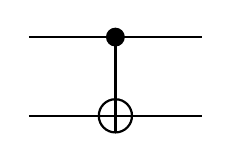
\begin{tikzpicture}[line width=0.8pt,
    control/.style={fill=black, draw=black, shape=circle, minimum size=6pt, inner sep=0pt},
    target/.style={draw, shape=circle, minimum size=12pt, inner sep=0pt}
]
% --- Qubit-Leitungen ---
\draw (-0.6,1) -- (1.6,1);  % obere Leitung
\draw (-0.6,0) -- (1.6,0);  % untere Leitung
% --- CNOT: Kontrollpunkt ---
\node[control] (ctrl) at (0.5,1) {};
% --- CNOT: Zielkreis mit Pluszeichen ---
\node[target] (targ) at (0.5,0) {};
\draw (0.5,-0.2) -- (0.5,0.2);   % vertikale Linie im Plus
\draw (0.3,0) -- (0.7,0);        % horizontale Linie im Plus
% --- Verbindungslinie zwischen Control und Target ---
\draw (ctrl) -- (targ);
% --- Untertitel ---
%\node at (0.5,-0.8) {\small Darstellung eines CNOT-Gatters (Controlled-NOT-Gatter)};
\end{tikzpicture}
\caption{Darstellung des CNOT-Gatters (nach \cite[S.178]{nielsen_quantum_2010})}
\end{figure} \\
CNOT-Gatter spielt eine zentrale Rolle in der Quantenlogik, da es im Zusammenspiel mit Ein-Qubit-Gattern eine zweistufige Unitarität bildet und sich daraus jeder beliebige Quantum-Schaltkreis bilden lässt. (Vgl. ebd. S.191) Ein Beispiel, bei dem das CNOT-Gatter zur Verschränkung beiträgt, ist bei der Erzeugung von Bell-Zuständen - dieses Thema wird in Unterkapitel \ref{sec:bell_zustand} erläutert. Darüber hinaus bilden CNOT-Gatter die Grundlage für komplexere Operationen wie bspw. beim Toffoli-Gatter (CCNOT). (Vgl. \cite[S.5f.]{abughanem_toffoli_2025})



\subsubsection{SWAP}
Ein SWAP-Gatter vertauscht den Zustand zweier Qubits. Formal entspricht es der Abbildung $|a,b\rangle \mapsto |b,a\rangle$ mit $a,b \in \{0,1\}$. In der Standardbasis $\{|00\rangle, |01\rangle, |10\rangle, |11\rangle\}$ ergibt sich daraus folgende Matrix:

\begin{equation}
U_{\text{SWAP}} =
\begin{pmatrix}
1 & 0 & 0 & 0 \\
0 & 0 & 1 & 0 \\
0 & 1 & 0 & 0 \\
0 & 0 & 0 & 1
\end{pmatrix}
\end{equation}
\\
Diese Matrix vertauscht $|01\rangle$ und $|10\rangle$, während $|00\rangle$ und $|11\rangle$ unverändert bleiben. (Vgl. \cite[S.79]{rieffel_quantum_2011}) Der Gatter ist unitär, selbstinvers ($U^2 = I$) und hermitesch ($U = U^\dagger$). Damit erfüllt er alle Bedingungen für eine physikalisch zulässige Quantenoperation. (Vgl. \cite[S.2]{gheorghiuStandardFormQudit2011})\\
\\
Eine direkte Realisierung des SWAP-Gatters ist auf vielen Hardwareplattformen nicht vorgesehen. Stattdessen lässt es sich durch eine Folge von drei CNOT-Gattern konstruieren:
\begin{figure}[h]
\centering
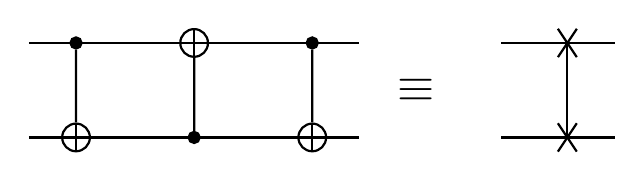
\begin{tikzpicture}[line width=0.8pt, scale=1.2,
    control/.style={fill=black, draw=black, shape=circle, minimum size=4pt, inner sep=0pt},
    target/.style={draw, shape=circle, minimum size=10pt, inner sep=0pt},
    cross/.style={line width=0.8pt}
]

% --- Linien links ---
\draw (0,1) -- (3.5,1); % obere Leitung
\draw (0,0) -- (3.5,0); % untere Leitung

% --- CNOT 1 (oben kontrolliert) ---
\node[control] (c1) at (0.5,1) {};
\node[target]  (t1) at (0.5,0) {};
\draw (c1) -- (t1);
\draw (0.5,0) -- ++(-0.15,0);
\draw (0.5,0) -- ++(0.15,0);
\draw (0.5,-0.15) -- (0.5,0.15);

% --- CNOT 2 (unten kontrolliert) ---
\node[control] (c2) at (1.75,0) {};
\node[target]  (t2) at (1.75,1) {};
\draw (c2) -- (t2);
\draw (1.75,1) -- ++(-0.15,0);
\draw (1.75,1) -- ++(0.15,0);
\draw (1.75,0.85) -- (1.75,1.15);

% --- CNOT 3 (oben kontrolliert) ---
\node[control] (c3) at (3,1) {};
\node[target]  (t3) at (3,0) {};
\draw (c3) -- (t3);
\draw (3,0) -- ++(-0.15,0);
\draw (3,0) -- ++(0.15,0);
\draw (3,-0.15) -- (3,0.15);

% --- Gleichheitszeichen ---
\node at (4.1,0.5) {\LARGE $\equiv$};

% --- Linien rechts (SWAP) ---
\draw (5,1) -- (6.2,1);
\draw (5,0) -- (6.2,0);

% --- SWAP Gatter (gekreuzte X) ---
\draw[cross] (5.6,1.15) -- (5.8,0.85);
\draw[cross] (5.6,0.85) -- (5.8,1.15);
\draw[cross] (5.6,-0.15) -- (5.8,0.15);
\draw[cross] (5.6,0.15) -- (5.8,-0.15);
\draw (5.7,1) -- (5.7,0);

\end{tikzpicture}
\caption{Zerlegung des SWAP-Gatters in drei CNOT-Gatter (nach \cite[S.~23]{rieffel_quantum_2011})}
\end{figure}
\\
Ein zentrales Einsatzgebiet ergibt sich in Systemen mit begrenzter Konnektivität. Wenn zwei Qubits, die miteinander interagieren sollen, nicht direkt gekoppelt sind, werden SWAP-Gatter eingesetzt, um Zustände über benachbarte Qubits hinweg zu verschieben. Dieses Vorgehen ist unter dem Begriff \emph{Qubit-Routing} bekannt. (Vgl. \cite[S.2f.]{molaviQubitMappingRouting2022}) Auch in der Quanten-Fourier-Transformation wird das SWAP-Gatter verwendet. Am Ende der Transformation wird die spiegelverkehrte Reihenfolge der Qubits mithilfe von SWAP-Gattern wiederhergestellt, indem jeweils Paare symmetrisch zur Mitte des Registers vertauscht werden. (Vgl. \cite[S.219]{nielsen_quantum_2010})

%(Qubit Mapping and Routing via MaxSAT, S.2f.)


%\subsection{CU-Gatter}
%\subsection{Quantenschaltungen}


\section{Erste Algorithmen}
Algorithmen in der klassischen Informatik basieren alle auf einer linearen, schrittweisen Verarbeitung von Daten. So kann ein Bit, mit dem Wert 1 in einem folgenden Rechenschritt entweder den Wert 0 annehmen oder seinen aktuellen Wert 1 behalten. In einem Quantencomputer hingegen, kann das QBit nach einer Transformation unendlich viele verschiedene Werte annehmen.\\
\\
Mit dem Wissen aus vorherigen Kapitel lassen sich bereits die ersten, einfachen Quantenalgorithmen entwerfen, welche theoretisch schneller auf Quantencomputer ausgeführt werden können oder sogar für klassische Computer unmöglich sind zu lösen. \\
\\
Dazu beleuchten wir die Herkunft moderner Quantencomputer und die ersten Quantenalgorithmen.

\subsection{Algorithmus von Deutsch} 

In einem Paper von 1985 stellt der Physiker David Deutsch die Idee eines universellen Quantencomputers vor. Dabei verbindet er Quantenmechanik mit der theoretischen Informatik und kritisiert die klassische Church-Turing-These, da sie physikalisch nicht vollständig sei. Er schlägt stattdessen die Church–Turing–Deutsch-These vor: Alles, was physikalisch berechenbar ist, kann von einem Quantencomputer simuliert werden.\\
\\
Zentral im Paper ist der Vorschlag eines konkreten Quantenalgorithmus, welcher heute als der Deutsch-Algorithmus bekannt ist. Dieser zeigt, dass Quantencomputer Probleme effizienter lösen können als klassische Rechner.  (Vgl. \cite{deutsch_quantum_1985}) \\
\\
Wir wollen herausfinden ob ein Münze echt oder gefälscht ist. Bei einer echten Münze zeigen beide Seiten unterschiedliche Motive. Ist die Münze eine Fälschung, sind die Seiten gleich. Um eine echte Münze von einer Fälschung unterscheiden zu können, muss zuerst die Vorderseite und danach die Rückseite überprüft werden. In einem Quantencomputer können wir beide Seiten gleichzeitig prüfen. Das Überprüfen der Münze können wir als folgende binäre Funktion darstellen.

$$f:\{0,1\} \rightarrow \{0,1\}$$. 

Der Algorithmus von Deutsch möchte herausfinden, ob $f$ konstant (d.h. $f(0)=f(1)$) oder balanciert (d.h. $f(0)\neq f(1)$) ist. Übertragen wir das auf die Überprüfung der Münze, ist in dem Fall $f(0) = f(1)$ die Münze eine Fälschung und in dem Fall $f(0) \neq f(1)$ die Münze echt. \\
\\
Ein klassischer Computer muss beide Werte $f(0)$ und $f(1)$ abfragen. \\
\\
Deutsch zeigt, dass ein Quantencomputer mit nur einer Abfrage an ein Quanten-Orakel die Antwort liefern kann. Ein Quantenorakel ist dabei eine unbelichtete Funktion, welche $n$-Bits als Eingabe und $m$-Bits als Ausgabe liefert. Man könnte das Orakel auch als "Black Box" bezeichnen, deren Funktionsweise für unser Problem nicht relevant ist. Es ist also egal wie ein Computer die Münze überprüft, solange das Ergebnis der Prüfung einer Seite richtig ist. \\
\\
Um das Problem mit der Münze zu lösen, müssen wir eines der Quantenbits in eine Superposition über beide möglichen Eingaben von $f$ versetzten. Danach wird das Orakel angewendet und wir bekommen ein Superposition über beide Funktionswerte zurück.\\
\\
Damit das Problem für einem Quantencomputer lösbar ist, müssen alle Rechenschritte umkehrbar sein. Da $f$ in dem konstanten Fall nicht reversible ist muss ein zweites Quantenbit für den Algorithmus verwenden werde. Daraus ergibt sich folgender Funktionsaufruf. Die Operation $\oplus$ entspricht dabei einem exklusiven Oder.

$$
U_f: \left|x\right\rangle\left| y\right\rangle \rightarrow  \left|x, y \oplus f(x)\right\rangle
$$\\
\\
Jetzt kann auf das Problem der Algorithmus von Deutsch angewendet werden. Dieser löst das Problem in folgenden 4 Schritten:

\begin{enumerate}
    \item Initialzustand: Zwei QBits im Zustand
$$\left|x\right\rangle\left|y\right\rangle \leftarrow  \left|0\right\rangle \left|1\right\rangle$$
\item Anwenden des Hadamard-Gatters auf beide QBits erzeugt Superposition:
$$
\left|x\right\rangle\left|y\right\rangle \leftarrow  H\left|x\right\rangle H\left|y\right\rangle
$$
\item Anwendung des Orakels $U_f$:
 $$
\left|x\right\rangle\left|y\right\rangle \leftarrow  U_f\left|x\right\rangle\left|y\right\rangle
$$
    Durch die vorbereitete Superposition des Zielregisters wird die Funktion $f(x)$ in die Phase codiert.
\item Nach erneuter Hadamard-Transformation misst man:
 \begin{itemize}
     \item Hat $\left|x\right\rangle\left|y\right\rangle$ den Wert $\left|0\right\rangle\left|1\right\rangle$: Funktion ist konstant oder die Münze ist eine Fälschung
     \item Hat $\left|x\right\rangle\left|y\right\rangle$ den Wert $\left|1\right\rangle\left|1\right\rangle$: Funktion ist balanciert oder die Münze ist echt
 \end{itemize}
\end{enumerate}

\begin{table}[h]
    \centering
    \renewcommand{\arraystretch}{1.5}
    \begin{tabular}{p{3cm} p{8cm}}
        \textbf{Schritt} & \textbf{Beschreibung} \\ \hline
        1. Initialzustand &
        Zwei QBits im Zustand:
        
        \(\left|x\right\rangle\left|y\right\rangle \gets \left|0\right\rangle \left|1\right\rangle\)
        \\

        2. Erzeugen einer Superposition &
        Anwenden des Hadamard-Gatters auf beide QBits erzeugt Superposition:
        
        \(\left|x\right\rangle\left|y\right\rangle \gets H\left|x\right\rangle H\left|y\right\rangle\)
        \\

        3. Anwenden des Quantenorakels \(U_f\) &
        Durch die vorbereitete Superposition des Zielregisters wird die Funktion \(f(x)\) in die Phase codiert:
        
        \(\left|x\right\rangle\left|y\right\rangle \gets U_f\left|x\right\rangle\left|y\right\rangle\)
        \\

        4. Messen &
        Nach erneuter Hadamard-Transformation misst man:
        \begin{itemize}

         \item Hat $\left|x\right\rangle\left|y\right\rangle$ den Wert $\left|0\right\rangle\left|1\right\rangle$: Funktion ist konstant oder die Münze ist eine Fälschung
    
         \item Hat $\left|x\right\rangle\left|y\right\rangle$ den Wert $\left|1\right\rangle\left|1\right\rangle$: Funktion ist balanciert oder die Münze ist echt
    
     \end{itemize}
    \end{tabular}
    \caption{Schritte des Deutsch-Algorithmus}
    \label{tab:deutsch_algorithmus}
\end{table}

Daraus folgt der Schaltkreis in Abbildung \ref{fig:deutsch-schaltkreis}.
\begin{figure}
    \centering
    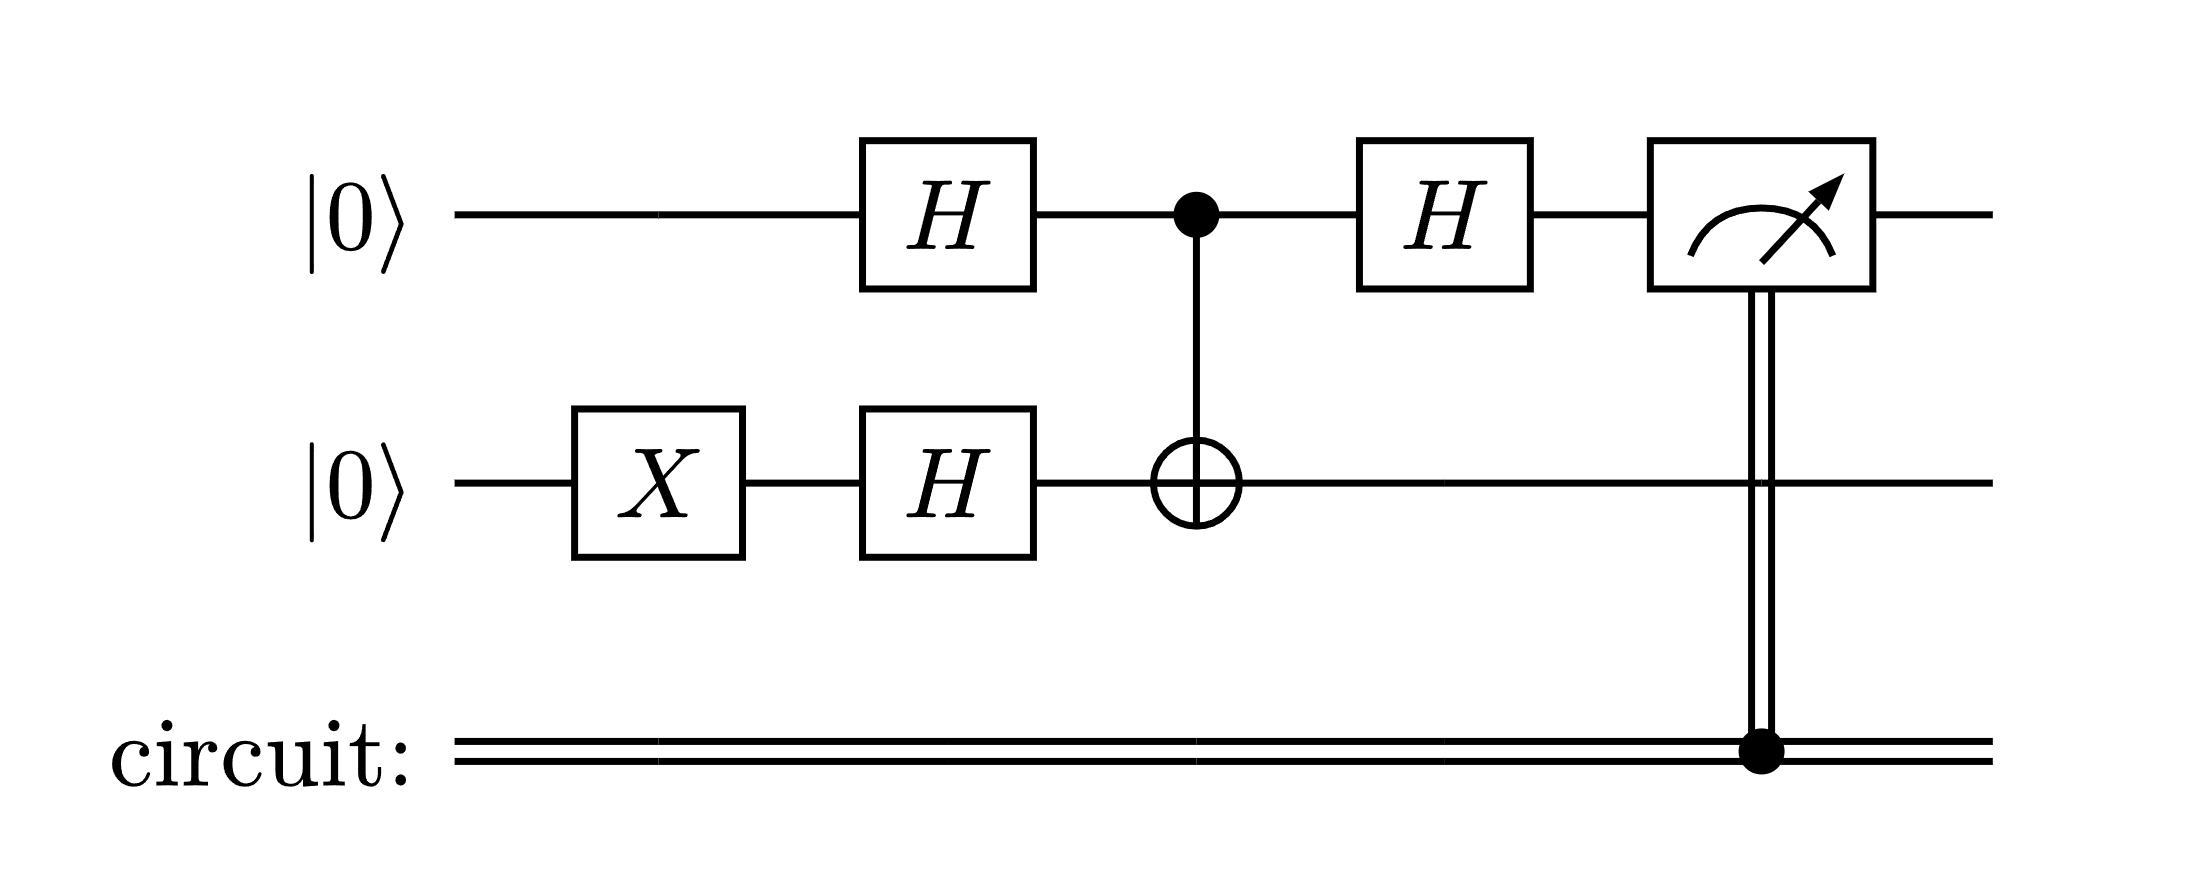
\includegraphics[width=1\linewidth]{images//quantum-information/deutsch schaltkreis.png}
    \caption{Schaltkreis: Deutsch-Algorithmus}
    \label{fig:deutsch-schaltkreis}
\end{figure}

Somit liefert Deutsch den ersten konkreten Algorithmus, welcher Quantenparallelität durch Superpositionen ausnutzt. Der von Deutsch vorgeschlagene Algorithmus ermöglicht es jedoch nur Probleme mit einem einzigen Eingabebit zu verarbeiten. Eine verallgemeinerte Version des Deutsch-Algorithmus lieferte David Deutsch zusammen mit Richard Jozsa ein paar Jahre später in dem Paper "Rapid solution of problems by quantum computation". (Vgl. \cite[S.33-37]{homeister_quantum_2022})

\subsection{Deutsch-Josza Algorithmus}\label{subsec_jasza}
Reale Probleme haben meist deutlich komplexere Strukturen und benötigen mehrere Eingabebits. Dazu entwickelten David Deutsch und Richard Jozsa eine Verallgemeinerung, welche als Deutsch-Jozsa-Algorithmus bekannt ist. Dieser erlaubt es, Funktionen mit beliebig vielen Eingabebits zu untersuchen und demonstriert erstmals einen exponentiellen Vorteil gegenüber klassischen Computern.\\
\\
Genau wie bei dem Deutsch-Algorithmus ist eine Funktion $f:\{0,1\}^n \rightarrow \{0,1\}$ gegeben. Dieses mal aber mit $n$-Bits als Eingabe. $f$ ist entweder konstant oder balanciert. Im balancierten Fall sind genau die Hälfte aller Ausgaben $0$ und die andere Hälfte $1$. (Vgl. \cite{deutsch_rapid_1992})\\
\\
Das Ziel bleibt unverändert. Es soll mit möglichst wenig Abfragen bestimmt werden, welcher der beiden Fälle vorliegt. Klassische Algorithmen benötigen für das Problem im schlimmsten Fall $2^{n-1}+1$ Abfragen, um Gewissheit zu erlangen. \\

Der Algorithmus läuft in folgenden Schritten ab:

\begin{enumerate}
\item Initialzustand:  Ein Register mit $n$ QBits im Zustand $\left|0\right\rangle^{\otimes n}$ und ein Hilfs-QBit im Zustand $\left|1\right\rangle$
\item Hadamard-Transformation auf alle QBits erzeugt eine Superposition:
$$
\left|x\right\rangle\left|y\right\rangle \leftarrow  H^{\otimes n}\left|0\right\rangle^{\otimes n} \otimes H\left|1\right\rangle
$$
\item Anwendung des Orakels $U_f$, das kohärent alle $2^n$ Eingaben verarbeitet:
$$
U_f \left|x\right\rangle\left|y\right\rangle = \left|x\right\rangle\left|y \oplus f(x)\right\rangle
$$
    Wie beim Deutsch-Algorithmus wird $f(x)$ in die Phase des Zustands eingeschrieben.
\item Erneute Hadamard-Transformation auf die ersten $n$ QBits.
\item Messung:
    \begin{itemize}
      \item Ergebnis $\left|0\right\rangle^{\oplus n}$ bedeutet die Funktion ist konstant
      \item Jedes andere Ergebnis bedeutet, die Funktion ist balanciert
    \end{itemize}
\end{enumerate}

\begin{table}[h]
    \centering
    \renewcommand{\arraystretch}{1.5}
    \begin{tabular}{p{3cm} p{8cm}}
        \textbf{Schritt} & \textbf{Beschreibung} \\ \hline

        1. Initialzustand &
        Ein Register mit \(n\) QBits im Zustand \(\left|0\right\rangle^{\otimes n}\) und ein Hilfs-QBit im Zustand \(\left|1\right\rangle\).
        \\

        2. Hadamard-Transformation &
        Anwenden von Hadamard-Gattern auf alle QBits erzeugt eine Superposition:
        
        \(\left|x\right\rangle\left|y\right\rangle \gets H^{\otimes n}\left|0\right\rangle^{\otimes n}\,\otimes\,H\left|1\right\rangle\).
        \\

        3. Anwendung des Orakels \(U_f\) &
        Das Orakel verarbeitet kohärent alle \(2^n\) möglichen Eingaben:
        
        \(
        U_f \left|x\right\rangle\left|y\right\rangle = \left|x\right\rangle\left|y \oplus f(x)\right\rangle.
        \)
        
        Wie beim Deutsch-Algorithmus wird \(f(x)\) in die Phase des Zustands eingeschrieben.
        \\

        4. Erneute Hadamard-Transformation &
        Auf die ersten \(n\) QBits wird erneut eine Hadamard-Transformation angewendet.
        \\

        5. Messung &
        Messung der ersten \(n\) QBits:
        \begin{itemize}
            \item Ergebnis \(\left|0\right\rangle^{\otimes n}\): Funktion ist konstant.
            \item Jedes andere Ergebnis: Funktion ist balanciert.
        \end{itemize}
        \\
    \end{tabular}
    \caption{Schritte des Deutsch-Jozsa-Algorithmus}
    \label{tab:deutsch_jozsa}
\end{table}


Abbildung \ref{fig:deutsch-jozsa-schaltung} zeigt einen entsprechenden Quantenschaltkreis mit 4 QBits. 
\begin{figure}
    \centering
    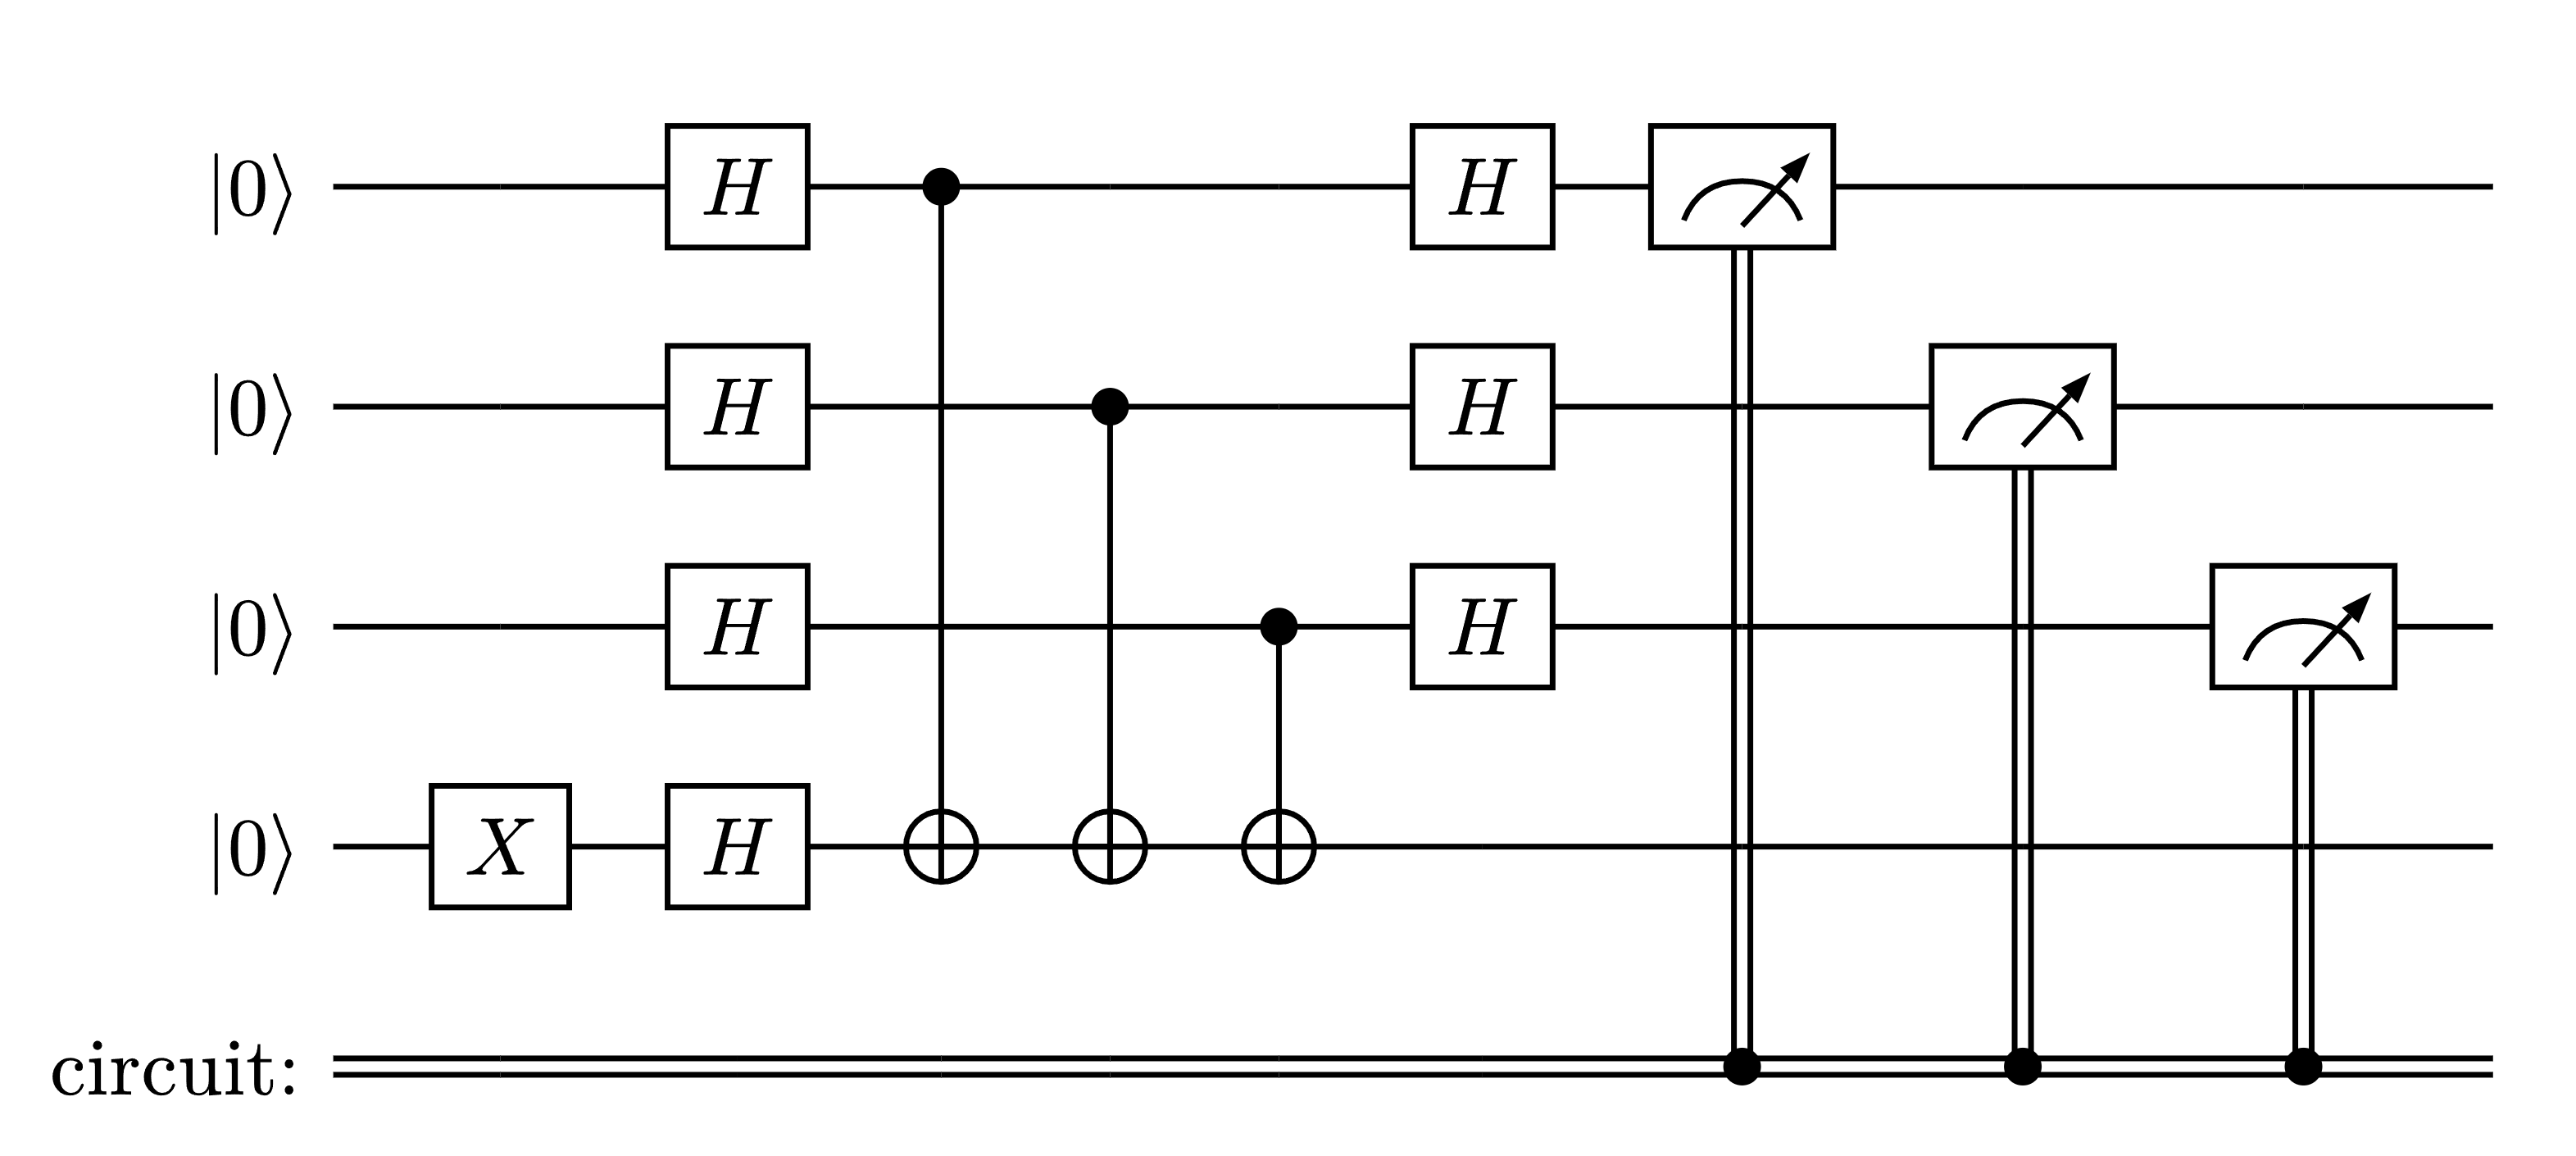
\includegraphics[width=1\linewidth]{images//quantum-information/deutsch-jozsa schaltkreis.png}
    \caption{Schaltkreis: Deutsch-Jozsa Algorithmus}
    \label{fig:deutsch-jozsa-schaltung}
\end{figure}

Das Besondere an dem Algorithmus ist, dass er das Ergebnis deterministisch und ohne Wahrscheinlichkeiten nach nur einer einzigen Orakelabfrage liefert. Durch Interferenz löschen sich bei balancierter Funktion die Amplituden für $\left|0\right\rangle^{\oplus n}$ vollständig aus. Nur im konstanten Fall bleibt sie erhalten. Somit liefert Deutsch und Jozsa den ersten theoretischen Beweis, dass Quantencomputer bei bestimmten Problemen klassischen Computern exponentiell überlegen sein können. (Vgl. \cite[S.62-66]{homeister_quantum_2022})





\section{Quantenverschränkung und Teleportation}

\subsection{Quantenverschränkung}
Quantenverschränkung ist ein Phänomen, bei dem zwei oder mehr Quantenobjekte sich in einem Zustand befinden, in dem sie, egal wie weit voneinander entfernt sie sind, gleich auf externe Reize reagieren. Solche Objekte, bei denen die Quantenverschränkung nachgewiesen werden konnte, sind Atome, Elementarteilchen wie Elektronen und Photonen, bis hin zu Kristallen.\\
\\
An einem Beispiel mit Elektronen lässt sich die Quantenverschränkung wie folgt erklären. Elektronen können sich in einem Zustand befinden, in dem sie keine eindeutige, exakte Position haben, sondern eine Menge an potentiellen Positionen. Diese potentiellen Positionen befinden sich alle im Umfeld der durchschnittlichen Position, dem Massenmittelpunkt des Elektrons, wie eine Wolke. Wenn von diesem Elektron seine Position gemessen wird, antwortet dieses Elektron auf die Messung mit einem zufälligen Wert. Bei den nächsten Messungen wird wiederum mit einem anderen zufälligen Wert geantwortet. Es besteht ein Indeterminismus. In diesem Zustand ist es sogar möglich, dass sich das Elektron, wegen dem Indeterminismus auch an zwei oder mehr Positionen gleichzeitig befindet. Und dieses Elektron, an zwei oder mehr Positionen gleichzeitig, reagiert auf Reize auf die gleiche Weise. Dies wurde im Doppelspaltexperiment von Thomas Young nachgewiesen, bei dem ein Elektron auf einen Reiz an der ersten Position an einem Young‘schen Spalt reagiert, und auf einen Reiz an der zweiten Position an einem anderen Young’schen Spalt reagiert.\\
\\
Obwohl es möglich ist, dass ein Quantenobjekt keine exakte Position hat, und ein weiteres mit dem ersten Quantenobjekt verbundenes, „verschränktes“ Quantenobjekt ebenfalls keine eindeutige Position hat, ist die Distanz zwischen den beiden Quantenobjekten klar bestimmt. Wenn man also die Position der beiden Quantenobjekte misst, erhält man für beide immer einen zufälligen Wert. Aber die Differenz der zufälligen Werte voneinander ist immer genau gleich. Das gilt immer, auch wenn die beiden Quantenobjekte sehr weit voneinander entfernt sind. Die Position eines Quantenobjekts selbst ist nicht wohlbestimmt, die Position im Bezug auf ein verbundenes, verschränktes Quantenobjekt hingegen schon. Dass sich ein Quantenobjekt „hier“ und „einer festen Distanz von hier“ gleichzeitig befindet, wird „Superposition“ genannt. Und dieser superpositionierte Zustand ist ein verschränkter Zustand.\\
\\
Die Verschränkung fixiert nicht nur die Distanz von zwei oder mehr Quantenobjekten voneinander, sondern auch weitere Variablen, z.B. die Geschwindigkeit. Sie haben die gleiche Geschwindigkeit, welche aber selbst nicht fest ist, sondern eine von einer Menge potentieller Geschwindigkeiten.\\
\\
(Vgl. \cite[S.83-88]{gisin_unbegreifliche_2014}) 

\subsection{Quantenteleportation - Übersicht}
Ein Objekt besteht aus Materie und physikalischem Zustand. Bei Quantenobjekten ist die Materie die Masse und permanente Attribute wie z.B. die elektrische Ladung bei Elektronen, bzw. die Energie bei massenlosen Quantenobjekten wie z.B. Photonen. Der physikalische Zustand besteht aus potentiellen, nicht eindeutigen Attributen, wie z.B. die potentiellen Positionen (Man denke die Positionen als Wolke um Massen-/ Energiemittelpunkt), die potentiellen Geschwindigkeiten bei Elektronen bzw. die potentiellen Schwingungsfrequenzen bei Photonen.\\
\\
In der Quantenteleportation wird der Zustand eines Quantenobjekts, der sog. Quantenzustand, ein Qubit, ohne das Durchlaufen einer Zwischenstrecke, also dem physischen Abstand der Quantenobjekte voneinander, von einer Position auf eine andere Position, vorausgesetzt, dass sich in dieser anderen Position ein Quantenobjekt derselben Art befindet, direkt versetzt. Die Masse bzw. Energie kann nicht teleportiert werden, weil dies das Prinzip der Unmöglichkeit von Kommunikation ohne Signalübertragung (Vgl. \cite[S.47-49]{gisin_unbegreifliche_2014})  verletzen würde. Dahingegen hat der Zustand weder eine Masse, noch eine Energie, denn sie ist potentiell – eine Wahrscheinlichkeit.\\
\\
Nach einer solchen Quantenteleportation verliert das Quantenobjekt seinen bisherigen Zustand und der neue Zustand entspricht dem Quantenzustand des zweiten Quantenobjekts vor der Quantenteleportation. Am Beispiel eines Photons kann man dies wie folgt erklären. Es gebe ein Photon mit gut strukturierter Polarisation. Bei solch einem Photon schwingt das elektrische Feld regelmäßig in eine bestimmte Richtung. Nach der Quantenteleportation verliert dieses Photon seine Struktur. Übrig bleibt ein depolarisiertes Photon, ein Photon mit strukturloser Polarisation, dessen elektrisches Feld unregelmäßig in alle Richtungen schwingt.\\
\\
Voraussetzung einer Quantenteleportation ist das Dasein einer Menge verschränkter Quantenobjekte. In der nächsten Subsektion wird hierüber genauer erläutert.\\
\\
(Vgl. \cite[S.124-128]{gisin_unbegreifliche_2014}) 


\subsection{Quantenteleportation - Hauptteil}
In einem theoretischen Szenario gibt ein Quantenobjekt eines Senders mit unbekanntem Quantenzustand bzw. Qubit \(\ket{\Phi}\). Dieser Qubit soll zu einem dritten Quantenobjekt eines Empfängers teleportiert werden. Der Sender ist im Besitz eines zweiten Quantenobjekts mit dem ursprünglichen Zustand \(\ket{\alpha_0}\), „Ancilla“ bzw. „Ancilla-Qubit“ genannt. Im ersten Schritt der Quantenteleportation bringt der Sender das Quantenobjekt mit dem Qubit \(\ket{\Phi}\) und das Quantenobjekt mit dem Ancilla-Qubit dazu, so miteinander zu interagieren, dass das erste Quantenobjekt in einen Standard Zustand \(\ket{\Phi_0}\), und das zweite Quantenobjekt in einen unbekannten Quantenzustand \(\ket{\alpha}\), welches die vollständige Information über \(\ket{\Phi}\) enthält, versetzt wird. Diese Interaktion ist eine gemeinsame Messung der Quantenzustände beider Quantenobjekte des Senders. Allerdings muss erwähnt werden, dass eine solche Messung nur ein positives Ergebnis liefert, wenn der Qubit \(\ket{\Phi}\) einem orthonormalen Set angehört. Dies bedeutet, dass die Qubit-Vektoren in diesem Set orthogonal zueinander sind, und gleichzeitig eine Norm von 1 haben. Im zweiten Schritt der Quantenteleportation wird dann die neue Ancilla, bzw. in anderen Worten das (positive) Ergebnis der Messung im ersten Schritt, an das Quantenobjekt des Empfängers gesendet, wonach der Empfänger die Qubit-Veränderung auslösende Interaktion vom Sender rückgängig machen kann, und somit eine Replikation des originalen Quantenobjekts mit dem Qubit \(\ket{\Phi}\) herstellen kann. Auf dieser Weise können Informationen von Quantenobjekten, also Quanteninformationen, ausgetauscht werden, ohne dass ein Quantenobjekt geklont wird, weil letzteres nach dem "No-Cloning-Theorem" (Vgl. \cite[S.77]{gisin_unbegreifliche_2014}) nicht möglich ist. Diese Methode der Quantenteleportation wird „spin-exchange“ genannt.\\
\\
(Vgl. \cite[S.1-2]{bennett_teleporting_1993})\\
\\
Am anfänglichen Zustand der „spin-exchange“ Methode sind das Quantenobjekt 2 auf der Senderseite und das Quantenobjekt 3 auf der Empfängerseite miteinander verschränkt. Durch die Interaktion auf Senderseite, wobei die Qubits der Quantenobjekte 1 und 2 verändert werden, wird die Verschränkung der Quantenobjekte 2 und 3 aufgehoben, und stattdessen die Quantenobjekte 1 und 2 verschränkt.\\
\\
(Vgl. \cite[S.2-3]{bennett_teleporting_1993})\\
\begin{figure}[h!]
    \centering
    \includegraphics[width=1.0\textwidth]{images/quantum-information/quantenverschränkung.png}
    \caption{Quantenobjekte als Würfel dargestellt}
    \label{fig:meinbild}
\end{figure}
\newpage
\noindent Mathematisch lässt sich der Prozess, wobei die Quantenobjekte in diesem Beispiel spin-\(\frac{1}{2}\) Partikel sind, mit folgenden Formeln darstellen:

\[ \ket{\Psi_{23}^{(-)}} = \sqrt{\frac{1}{2}} (\ket{\uparrow_2}\ket{\downarrow_3} + \ket{{\downarrow_2}\ket{\uparrow_3}}) \]
\\
Das zweite Quantenobjekt vom Sender (2) und das Quantenobjekt vom Empfänger (3) befinden sich in einem verschränkten Zustand. Dies ist die Ausgangssituation.

\[ \ket{\Psi_{12}^{(+)}} = \sqrt{\frac{1}{2}} (\ket{\uparrow_1}\ket{\downarrow_2} + \ket{{\downarrow_1}\ket{\uparrow_2}}) \]
\[ \ket{\Phi_{12}^{(\pm)}} = \sqrt{\frac{1}{2}} (\ket{\uparrow_1}\ket{\uparrow_2} \pm \ket{{\downarrow_1}\ket{\downarrow_2}}) \]
\\
Nun findet die gemeinsame Messung der beiden Quantenobjekte des Senders statt. Die vier sich in den Formeln befindenden Zustände bilden eine orthonormale Basis für die Quantenobjekte 1 und 2. Hiermit ist die Verschränkung der Quantenobjekte 2 und 3 aufgehoben, und stattdessen sind 1 und 2 verschränkt.

\[ \ket{\Phi} = \ket{\Phi_1} = a{\uparrow_1} + b{\downarrow_1} \]
\\
Für einfache Verständlichkeit wird der unbekannte Originalzustand von Quantenobjekt 1, \(\ket{\Phi}\), so geschrieben. Dabei ist \(|a|^2 + |b|^2 = 1\).\\
\\
(Vgl. \cite[S.2]{bennett_teleporting_1993})

\subsection{Quantenkommunikation per Quantenverschränkung}
In der Quantenkommunikation bzw. im Quanteninformationstransfer innerhalb eines Quantennetzwerks werden Qubits bzw. Quantenzustände über Quantenkanäle gesendet. Quantenkanäle verbinden entfernte Knoten in einem solchen Netzwerk. Diese Quantenkanäle haben eine sog. Absorptionslänge. Die Länge der Quantenkanäle, und damit die maximale Distanz zweier miteinander verbundenen Knoten in einem Quantennetzwerk, ist nur auf wenige Vielfache der Absorptionslänge begrenzt. Dies führt zum Problem, dass Quantenkanäle „eng“ und „laut“ (Originaltext „noisy“) sind, und die transportierten Qubits sich miteinander verschränken können, was zu einem Übertragungsfehler führen könnte.\\
\\
Eine Lösung, die Wahrscheinlichkeit solcher Übertrangungsfehler zu reduzieren, mit Hinnahme von einer größeren Menge an benötigten Ressourcen, ist es, einzelne Qubits in einen konkatenierten Quantencode (z.B. einen verschränkten Zustand einer Vielzahl von Qubits) zu kodieren, und Operationen an diesem Code durchzuführen, während es durch den Quantenkanal übertragen wird. Dies wird „Verschränkungsreinigung“ (vom Eng. „entanglement purification“) genannt und ermöglicht möglichst unverfälschten Quanteninformationstransfer und sichere Quantenkryptographie in „engen“ und „lauten“ Quantenkanälen.\\
\\
Und um unverfälschten Quanteninformationstransfer auch über längere Quantenkanäle sicherzustellen, kann ein Schema verwendet werden, wobei sog. „Quantenrepeater“ einen langen Quantenkanal in kürzere Segmente aufteilen, und die Verschränkungen separat bereinigen, bevor diese wieder aneinander gehängt werden. Im Übergang von einem Segment zum nächsten werden Quantenkorrelationen aufgebaut, basieren auf Korrelationen die innerhalb der einzelnen Segmente existieren.\\
\\
(Vgl. \cite[S.1-2]{dur_quantum_1999})

\subsection{Quantenteleportation in Quantencomputern}
Die Informationen in den folgenden Abschnitten befinden sich in der Quelle (Vgl. \cite[S.1-2]{gottesman_quantum_1999}).\\
\\
Die Wissenschaftler Daniel Gottesman und Isaac Chuang stellen eine Technik, eine Verallgemeinerung von Quantenteleportation vor, welche Quantenberechnung in Quantencomputern effizient und ressourcenarm zulässt. Dadurch werden bekannte fehlertolerante Protokolle für Quantenberechnung vereinigt. Mit dieser Technik der Quantenteleportation sollen Quanteninformationen in einen neuen Zustand transformiert werden. Dies ähnelt der Wirkung eines Quantengatters.\\
\\
Zwei Qubits werden durch ein CNOT (controlled NOT) Gatter (gate) teleportiert. Ein CNOT gate ist eine Komponente, die zwei verschränkte Qubits in einem Bell-Zustand (Zustand, in dem zwei Qubits maximal miteinander verschränkt sind; mehr dazu in Subsektion 1.5.1) aufnimmt und den zweiten Qubit, den sog. „target“ Qubit dreht, wenn der erste Qubit, das sog. „control“ Qubit, einen Wert von \(\ket{1}\) hat. Beim Durchgang werden Pauli-Matrix Operationen durchgeführt, welche die Quanteninformationen auf einen dritten Qubit übertragen.\\
\begin{figure}[h!]
    \centering
    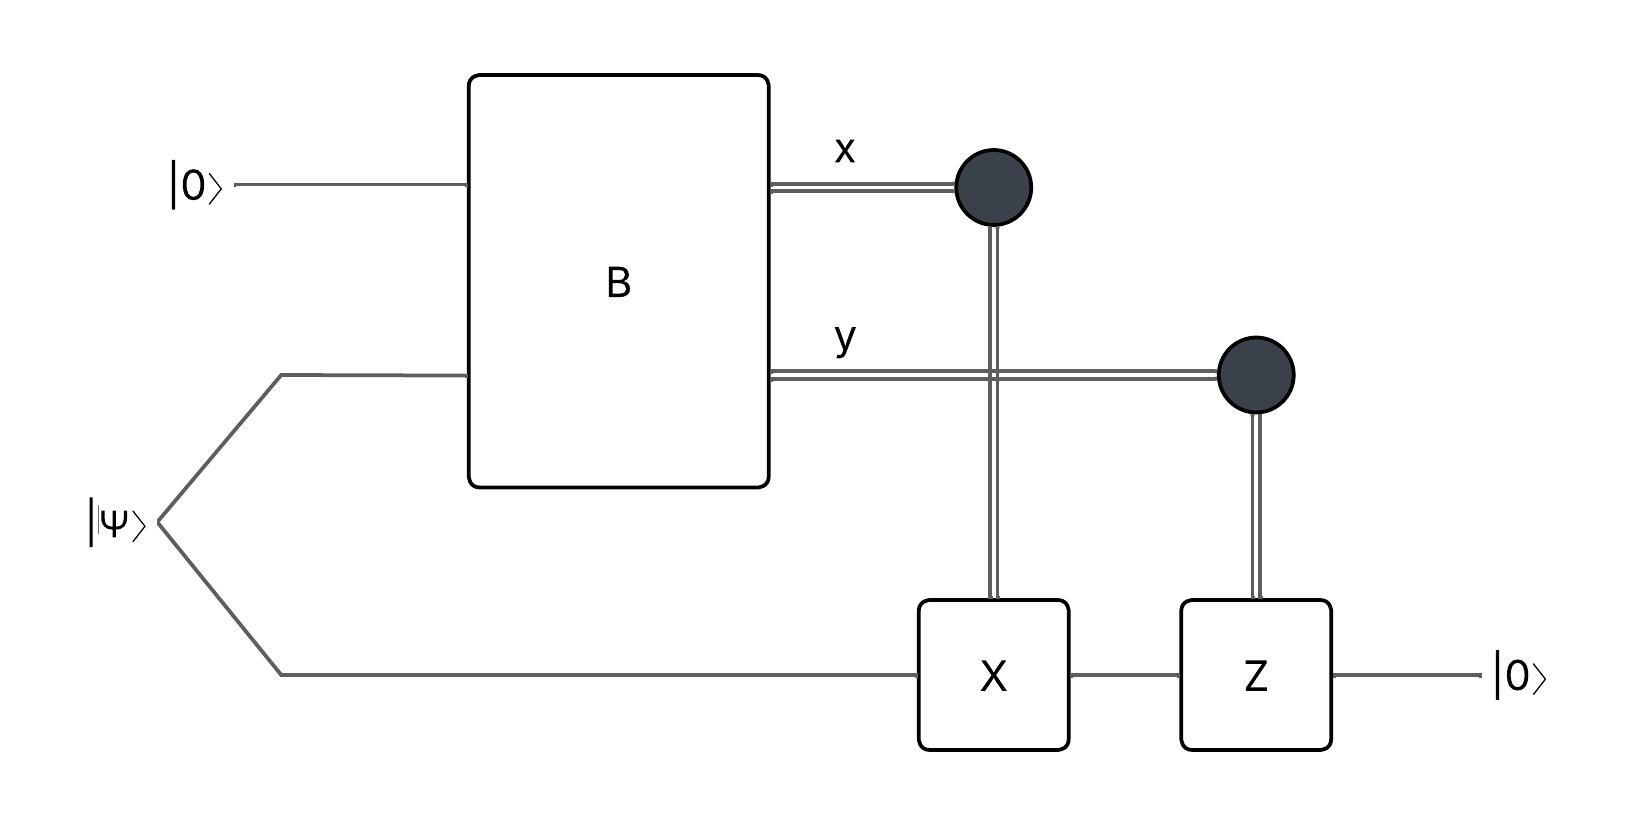
\includegraphics[width=1.0\textwidth]{images/quantum-information/quantenteleportation_cnot_1.jpeg}
    \caption{Zeitstrahl von links nach rechts. B = Bell-Zustand, X Y Z = Pauli Operatoren, \(\ket{0}\) = Zustand des Sender-Qubits, der an den Empfänger-Qubit übertragen werden soll}
    \label{fig:meinbild}
\end{figure}
\newpage
\noindent Dieses Prinzip kann leicht modifiziert werden. Die modifizierte Variante erlaubt es, vier Qubits, wovon jeweils zwei verschränkt sind, durchzulassen und anhand von Pauli-Matrix Operationen zu transformieren. Die zwei Paare von Verschränkungen sind vorerst getrennt. Eines enthält den „target“ Qubit \(\ket{\alpha}\), das andere den „control“ Qubit \(\ket{\beta}\). Der „target“ Qubit wird gedreht, wenn der „control“ Qubit einen Wert von \(\ket{1}\) hat. Es stehen 4 Rechenoperationen (I, X, Y, Z) zur Verfügung. Welche Operationen auf die Qubits der Verschränkungen angewendet werden, ist vom Zufall bestimmt. Zwei Qubits \(\ket{out}\), welche die Quanteninformationen von \(\ket{\alpha}\) und \(\ket{\beta}\) enthalten, wobei \(\ket{out}\) = CNOT\(\ket{\beta}\)\(\ket{\alpha}\), kommen aus den CNOT gate am Ende als Output heraus.\\
\begin{figure}[h!]
    \centering
    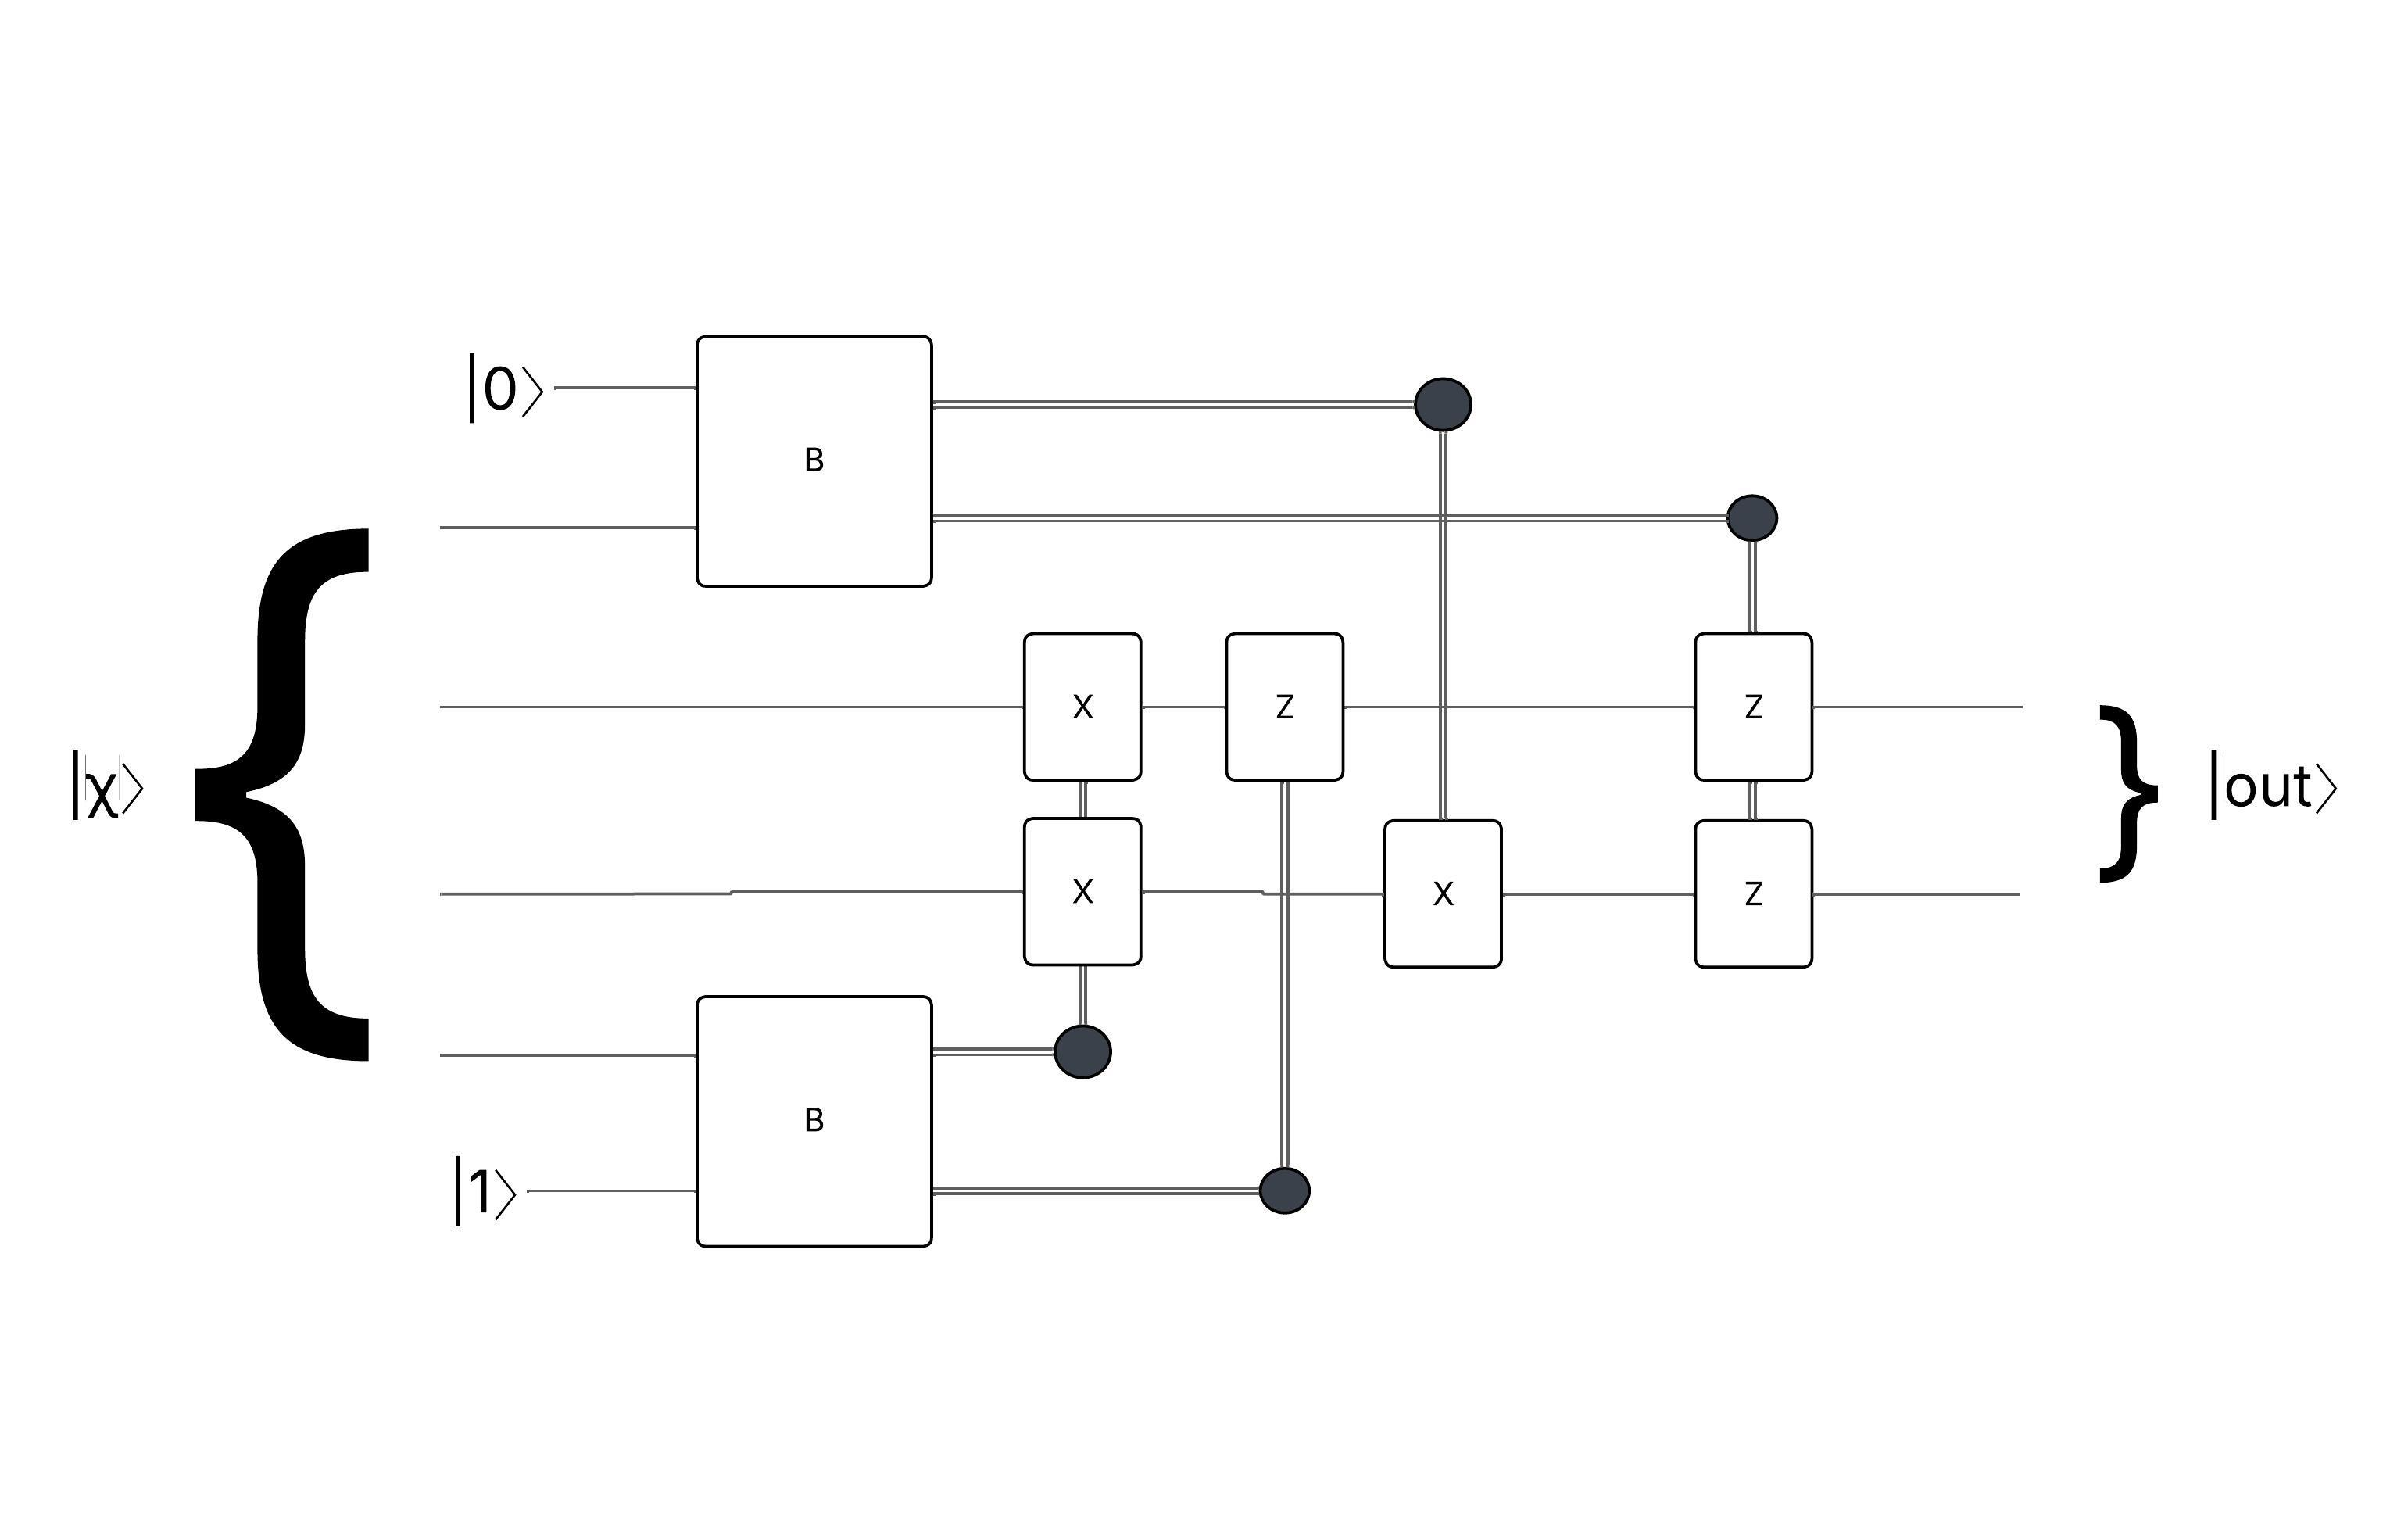
\includegraphics[width=1.0\textwidth]{images/quantum-information/quantenteleportation_cnot_2.jpeg}
    \caption{Zeitstrahl von links nach rechts. B = Bell-Zustand, X Y Z = Pauli Operatoren, \(\ket{\chi}\) = Ausgangszustand für Operation}
    \label{fig:meinbild}
\end{figure}
\newpage
\noindent Eine andere modifizierte Variante ist eine, bei der ein CNOT gate zwischen zwei Qubits von zwei unterschiedlichen verschränkten Qubit Paaren geöffnet wird. Der Output von solch einem Gatter kann verwendet werden, um den Zustand \(\ket{\chi}\) der vorherigen Abbildung zu bilden, von dem in einer Quantenteleportation mit zwei Verschränkungen Gebrauch gemacht wird. \(\ket{\chi}\) kann so erzeugt werden, oder durch eine Quantenteleportation zwischen zwei GHZ (Greenberger Horne Zellinger) Zuständen. Ein GHZ Zustand ist eine Verschränkung von drei Quantenobjekten.\\
\begin{figure}[h!]
    \centering
    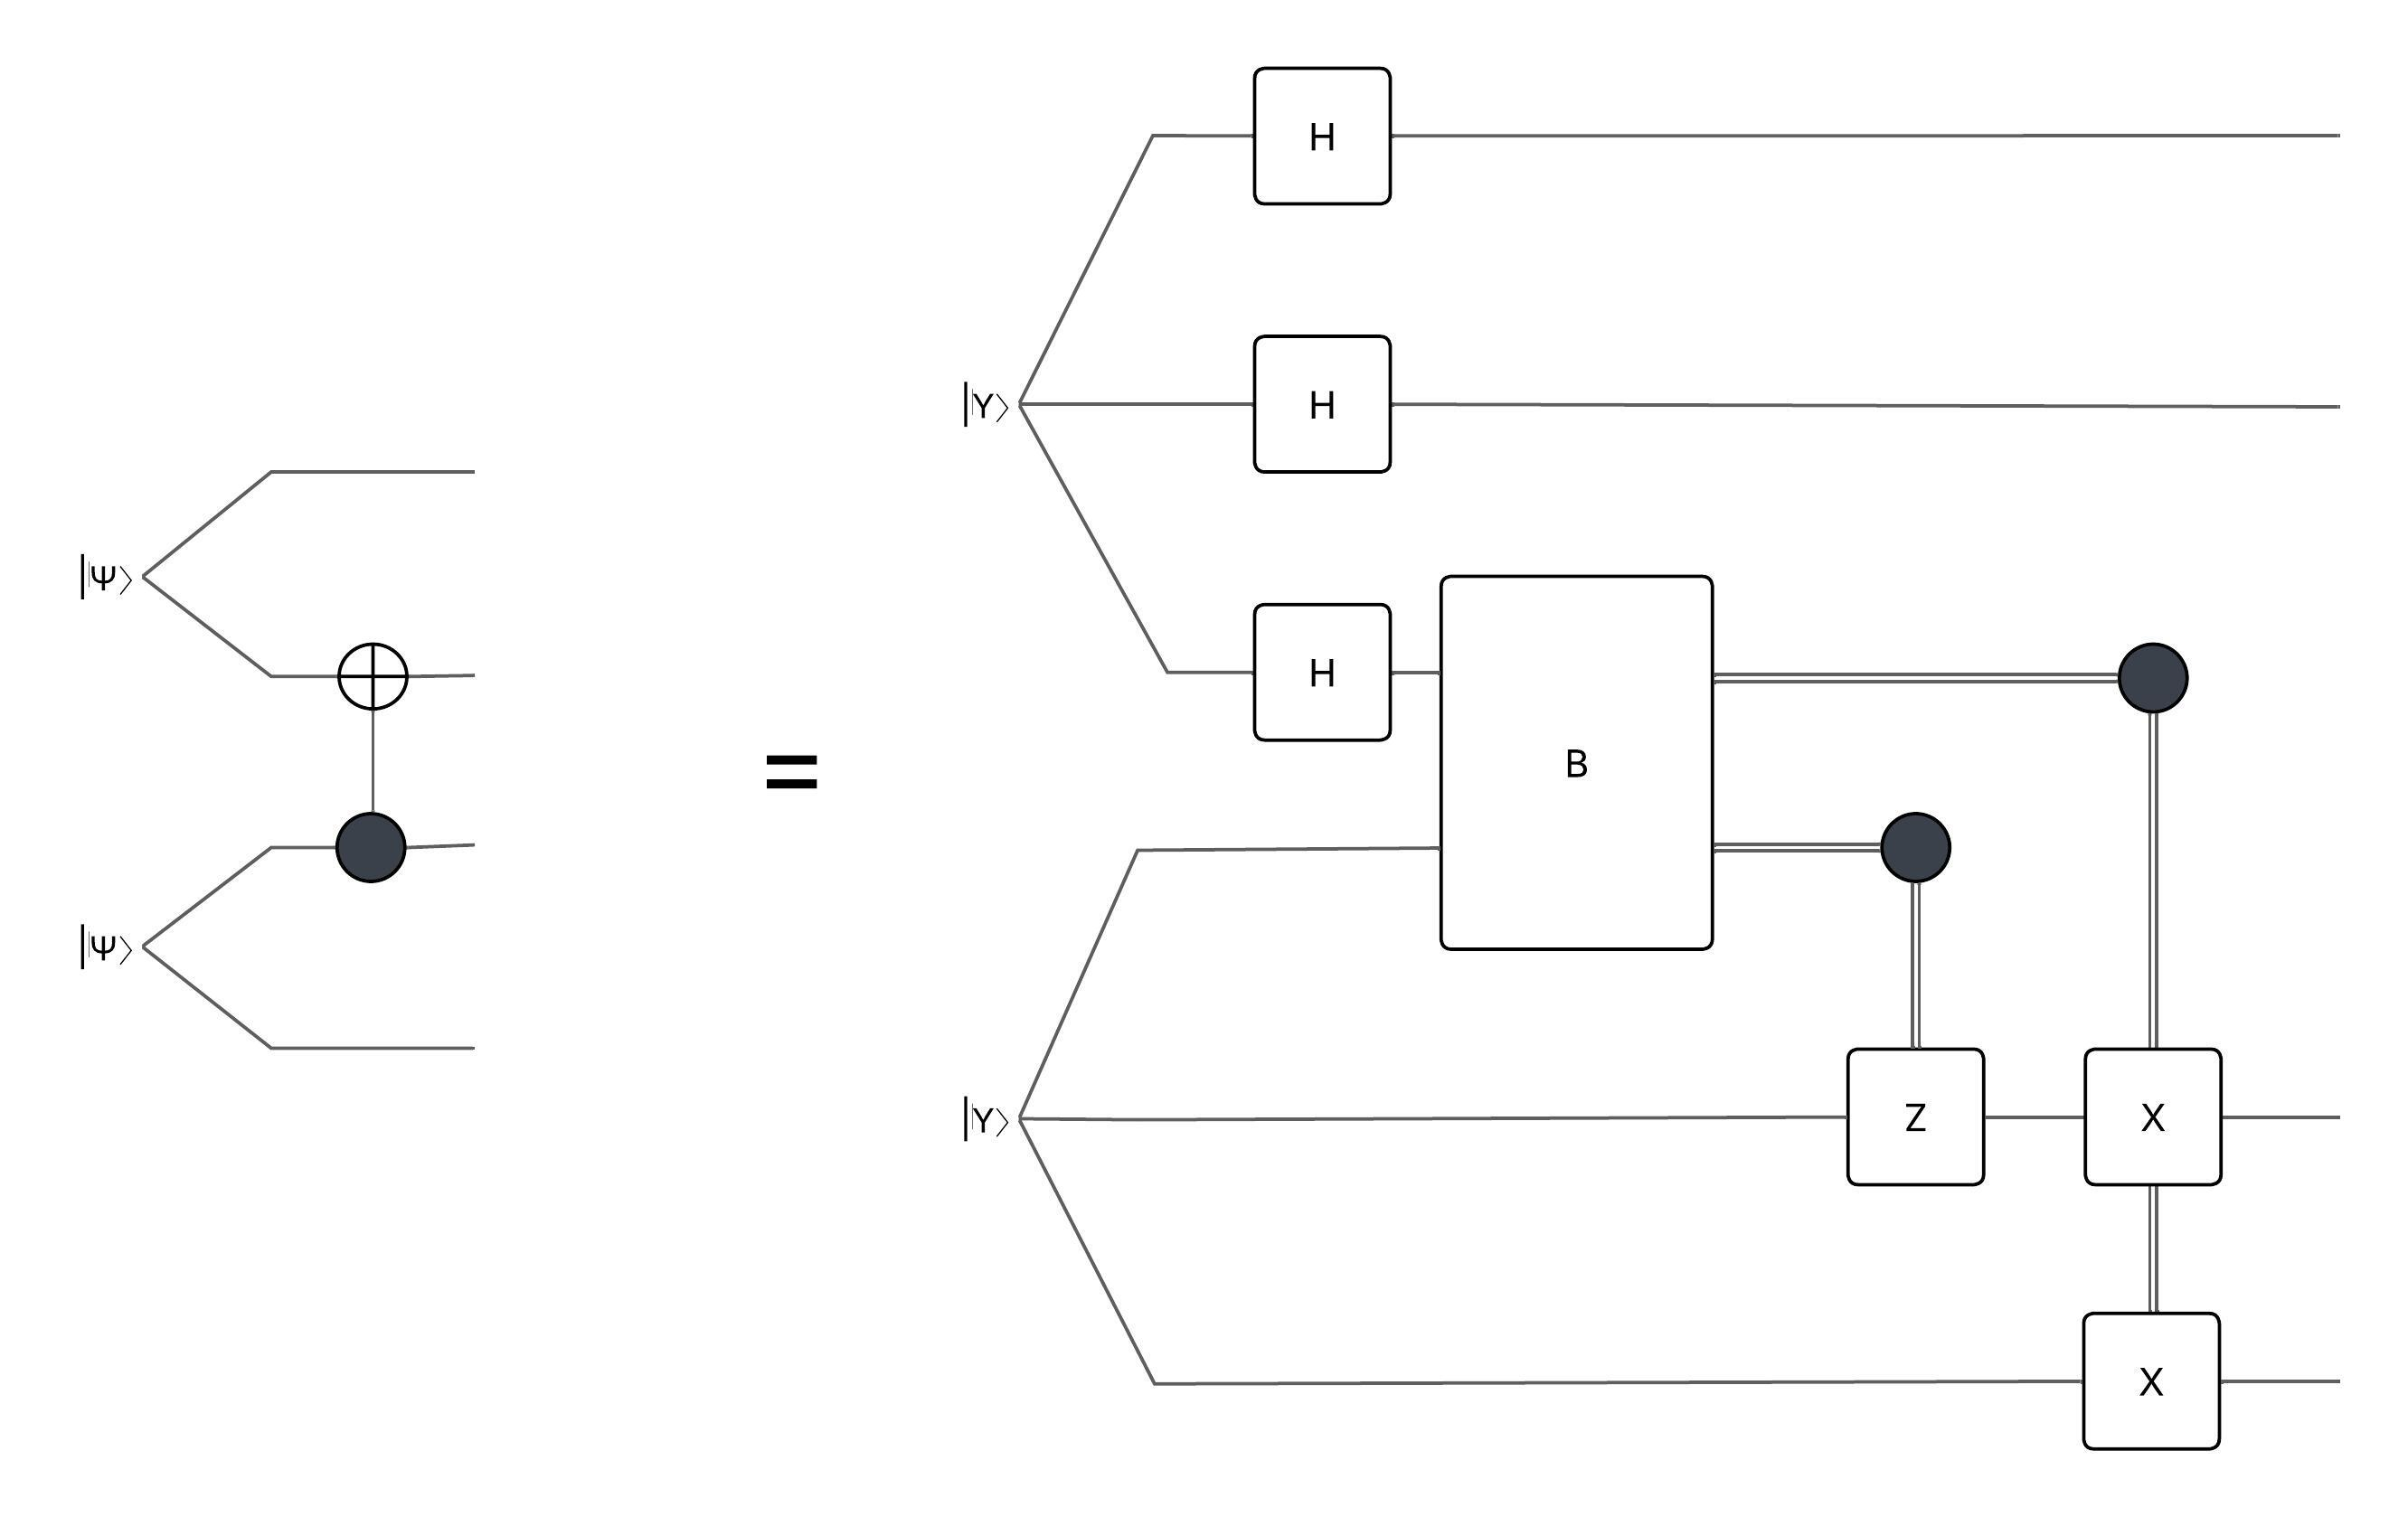
\includegraphics[width=1.0\textwidth]{images/quantum-information/quantenteleportation_cnot_3.jpeg}
    \caption{Zeitstrahl von links nach rechts. \(\ket{\Upsilon}\) = GHZ Zustand, H = Hadamard gate (für Hadamard Transformation), B = Bell-Zustand, X Z = Pauli Operatoren}
    \label{fig:meinbild}
\end{figure}
\newpage

\subsection{Bedeutung für Quantenkommunikation}
Wie Anhand der wissenschaftlichen Artikel von Bennett, Brassard et. al., sowie Gottesmann und Chuang gezeigt wurde, sind Quantenverschränkung und Quantenteleportation die Prinzipien, durch die es zu einem Quanteninformationstransfer kommen kann. Daraus kann man schließen, dass beide Prinzipien eine sehr wichtige Bedeutung für Quantenkommunikation haben.

\section{Fehlerkorrektur}
Qubits sind sehr fehleranfällig (mehr dazu ggf im Kapitel über physikalische Realisierung?). Im Gegensatz zu konventionellen Bits gestaltet sich die Fehlerkorrektur als schwieriger. Während konventionelle Bits kopiert und ausgelesen werden können, ist das bei Qubits nicht möglich, weil deren Superposition kollabieren würde, wenn man sie liest. Deshalb werden spezielle Quantenfehlerkorrekturverfahren entwickelt, die Fehler erkennen und beheben, ohne den Zustand der Qubits direkt zu messen. Diese Verfahren nutzen dabei die Verschränkung mehrerer Qubits, um Fehler zu detektieren und zu korrigieren, was allerdings einen erheblichen Mehraufwand an Qubits und Rechenressourcen erfordert.

In der Fehlerkorrektur sind insbesondere \emph{logische Qubits} wichtig. Ein logisches Qubit ist eine fehlerkorrigierte Version eines Qubits, die durch die Kodierung mehrerer physikalischer Qubits entsteht. Während ein physikalisches Qubit die tatsächliche quantenmechanische Implementierung darstellt, bildet ein logisches Qubit eine abstrakte Einheit, die durch redundante Kodierung vor Fehlern geschützt ist.

Die Funktionsweise basiert auf der Verteilung der Quanteninformation auf mehrere physikalische Qubits. Durch diese Redundanz können Fehler in einzelnen physikalischen Qubits erkannt und korrigiert werden, ohne die im logischen Qubit gespeicherte Information zu zerstören. 

Der Aufwand für die Implementierung logischer Qubits ist erheblich. Je nach verwendetem Fehlerkorrekturverfahren können hunderte oder sogar tausende physikalische Qubits erforderlich sein, um ein einzelnes logisches Qubit zu realisieren. Dieser Mehraufwand führt jedoch zu einer drastischen Verbesserung der Fehlerrate. Aktuelle Forschungsergebnisse zeigen, dass logische Qubits Fehlerarten aufweisen können, die um mehrere Größenordnungen niedriger sind als die ihrer physikalischen Komponenten. (vgl. \cite{divincenzoTopicsQuantumComputers1996}, \cite[426 ff.]{nielsen_quantum_2010}, \cite{ibm_research_team_introduction_nodate}).


\subsection{Beispiel: Bit-Flip}
Ein klassisches Beispiel für einen Fehler ist ein \emph{Bit-Flip}. Ein Bit-Flip liegt vor, wenn sich der Zustand eines Bits durch zum Beispiel kosmische Strahlung ungewollt ändert. Zur Fehlerkorrektur kann im Quantencomputing dann der sogenannte \emph{Bit-Flip-Code} verwendet werden. Dieser demonstriert hier das Grundprinzip logischer Qubits. Hierbei wird ein einzelnes logisches Qubit durch drei physikalische Qubits kodiert. Die Basiszustände werden dabei wie folgt abgebildet:

\begin{align}
\ket{0}_\text{logisch} &\rightarrow \ket{000}, \\
\ket{1}_\text{logisch} &\rightarrow \ket{111}.
\end{align}
Ein allgemeiner Qubit-Zustand
\begin{equation}
\ket{\psi} = \alpha \ket{0} + \beta \ket{1}
\end{equation}
wird somit als logischer Zustand kodiert zu:
\begin{equation}
\ket{\psi}_\text{logisch} = \alpha \ket{000} + \beta \ket{111}.
\end{equation}

Tritt ein Bit-Flip-Fehler auf einem der drei Qubits auf, entstehen fehlerhafte Zustände wie $\ket{001}$, $\ket{010}$ oder $\ket{100}$. Diese können durch eine \emph{Paritätsmessungen} erkannt und anschließend korrigiert werden, ohne die Amplituden $\alpha$ und $\beta$ zu zerstören.

Parität beschreibt in diesem Kontext, ob zwei Qubits denselben Zustand haben (also beide $\ket{0}$ oder beide $\ket{1}$) oder verschieden sind. Formal misst man die Parität zweier Qubits $i$ und $j$ durch den Operator:

\begin{equation}
 Z_i \cdot Z_j   
 \label{equ:parität_qubits}
\end{equation}


wobei $Z$ der Pauli-Z-Operator ist (vgl. Formel \ref{equ:pauli_matrizen}.

In der Praxis verwendet man ein Hilfsqubit (Ancilla), um diese Paritätsinformation indirekt zu messen. Der Ablauf ist wie folgt:

\begin{enumerate}
    \item Initialisiere das Ancilla-Qubit in Zustand $\ket{0}$.
    \item Wende zwei CNOT-Gatter an (vgl. Kapitel \ref{subsec:cnot_gatter}): 
    \begin{itemize}
        \item CNOT von Qubit $i$ auf das Ancilla-Qubit,
        \item CNOT von Qubit $j$ auf dasselbe Ancilla-Qubit.
    \end{itemize}
    \item Messe das Ancilla-Qubit in der Computational-Basis.
\end{enumerate}

Das Messergebnis liefert die Parität:
\begin{itemize}
    \item Ergebnis $\ket{0}$: Qubits $i$ und $j$ haben gleiche Parität ($\ket{00}$ oder $\ket{11}$),
    \item Ergebnis $\ket{1}$: Qubits haben unterschiedliche Parität ($\ket{01}$ oder $\ket{10}$).
\end{itemize}

Durch zwei Paritätsmessungen (z.B. zwischen Qubit 1–2 und 2–3) lässt sich ein einzelner Fehler eindeutig lokalisieren:

\begin{table}[h]
    \centering
\begin{tabular}{|c|c|c|}
\hline
Parität 1–2 & Parität 2–3 & Fehler in Qubit \\
\hline
gleich      & gleich      & keiner \\
ungleich    & gleich      & Qubit 1 \\
gleich      & ungleich    & Qubit 3 \\
ungleich    & ungleich    & Qubit 2 \\
\hline
\end{tabular}
   \label{tab:felherkorrektur}
\caption{Lokalisierung eines Fehlers in einem 3-Qubit-Sytems}
\end{table}


Das folgende Schaltbild zeigt die Paritätsmessung zwischen zwei Qubits mithilfe eines Ancilla-Qubits:

Sobald durch die Paritätsmessungen das fehlerhafte Qubit eindeutig identifiziert wurde (siehe Tabelle), wird der Fehler durch Anwendung eines Pauli-X-Gatters (Bit-Flip) auf das betroffene Qubit korrigiert. Das X-Gatter ist definiert als:

\[
X = \begin{pmatrix}
0 & 1 \\
1 & 0
\end{pmatrix},
\]

und wirkt auf die Basiszustände wie folgt:
\[
X\ket{0} = \ket{1}, \qquad X\ket{1} = \ket{0}.
\]

Beispielsweise:
\begin{itemize}
    \item Wenn Qubit 1 als fehlerhaft erkannt wurde (z.\,B. Zustand $\ket{100}$), wendet man $X$ auf Qubit 1 an:
    \[
    X_1\left( \alpha\ket{100} + \beta\ket{011} \right) = \alpha\ket{000} + \beta\ket{111}.
    \]
    \item Entsprechend für Qubit 2 oder 3.
\end{itemize}

Nach der Korrektur ist der logische Zustand wiederhergestellt:
\[
\ket{\psi}_\text{logisch} = \alpha\ket{000} + \beta\ket{111}.
\]

Die ursprüngliche Quanteninformation bleibt somit erhalten, obwohl ein physikalischer Fehler aufgetreten ist. Der Bit-Flip-Code demonstriert damit, wie Quantenfehler durch Redundanz und geeignete Messprotokolle erkannt und korrigiert werden können – ein grundlegendes Prinzip aller Quantenfehlerkorrekturverfahren. (vgl. \cite[426 ff.]{nielsen_quantum_2010})

\section{Bell-Zustand}\label{sec:bell_zustand}
Um die theoretischen Grundlagen der Quanteninformation greifbarer zu machen, bietet sich der Bell-Zustand als anschauliches Beispiel an. Er veranschaulicht zentrale Konzepte wie Quantenverschränkung und Nichtlokalität und bildet die Grundlage für viele Anwendungen in der Quantenkommunikation und -verarbeitung. Im Folgenden wird der Bell-Zustand näher erläutert, seine mathematische Darstellung vorgestellt und seine Bedeutung anhand konkreter Experimente und Anwendungen verdeutlicht.

\subsection{Was ist ein Bell-Zustand?}
Bell-Zustände sind spezielle Zustände in der Quantenmechanik, in denen zwei Teilchen maximal miteinander verschränkt sind. Das bedeutet: Ihre Zustände hängen so stark zusammen, dass man sie nicht unabhängig voneinander beschreiben kann – selbst, wenn die Teilchen physisch weit voneinander entfernt sind. Benannt ist der Bell-Zustand nach dem Physiker John S. Bell. Dieser zeigte im Jahre 1964 auf, dass die Vorhersagen der Quantenmechanik im Widerspruch zu den Prinzipien des lokalen Realismus stehen – also der Vorstellung, dass Informationen nicht schneller als Licht übertragen werden können und physikalische Größen vor der Messung bereits festgelegt sind. (Vgl. \cite[S.195]{bell_einstein_1964})
\\


Mit der von John S. Bell formulierten Bell-Ungleichung entwickelte Bell ein mathematisches Kriterium, mit dem sich klassische und quantenmechanische Theorien experimentell unterscheiden lassen. Die Quantenmechanik sagt unter bestimmten Bedingungen eine Verletzung der nach John S. Bell benannten Bell-Ungleichung voraus. Belegt wurde dies in zahlreichen Experimenten ab 1972, den sogenannten Bell-Test. Seitdem wurde die Verletzung der Bell-Ungleichung in zahlreichen Experimenten mit verschränkten Teilchenpaaren eindeutig nachgewiesen. In allen Fällen bestätigten die Ergebnisse die Vorhersagen der Quantenmechanik. 
(Vgl. \cite[S.53-59]{homeister_quantum_2022})

\subsection{Die vier Bell-Zustände}
Insgesamt existieren vier verschiedene Bell-Zustände, die eine Situation maximaler Verschränkung zwischen zwei Qubits beschreiben. Das heißt: Wird der Zustand eines Qubits gemessen, ist das Ergebnis des anderen automatisch bestimmt. Unabhängig von der Entfernung der Qubits voneinander. (Vgl. \cite[S.53-55]{homeister_quantum_2022}) 

\[
\begin{aligned}
\ket{\Phi^+} &= \frac{1}{\sqrt{2}} (\ket{00} + \ket{11}), \\
\ket{\Phi^-} &= \frac{1}{\sqrt{2}} (\ket{00} - \ket{11}), \\
\ket{\Psi^+} &= \frac{1}{\sqrt{2}} (\ket{01} + \ket{10}), \\
\ket{\Psi^-} &= \frac{1}{\sqrt{2}} (\ket{01} - \ket{10}).
\end{aligned}
\]

Mathematisch gibt es genau vier dieser Zustände, weil ein System aus zwei Qubits einen vierdimensionalen Zustandsraum besitzt. Die Bell-Zustände bilden darin eine vollständige Basis aller maximal verschränkten Zustände. Das heißt: Jede mögliche maximale Verschränkung zwischen zwei Qubits lässt sich als Kombination dieser vier Zustände ausdrücken.
\\


Die theoretischen Eigenschaften dieser Zustände lassen sich nicht nur mathematisch beschreiben, sondern auch ganz konkret auf Quantencomputern beobachten. In einer Simulation mit der IBM Quantum Learning Platform wurden hierfür zwei Qubits gezielt in einen verschränkten Zustand überführt. Das anschließende Messergebnis zeigt deutlich das charakteristische Verhalten eines Bell-Zustands: Es treten ausschließlich die Zustände \(\ket{00}\) und \(\ket{11}\) auf – jeweils mit 50\,\% Wahrscheinlichkeit. Die Kombinationen \(\ket{01}\) und \(\ket{10}\), bei denen sich die Qubits unterscheiden würden, wurden hingegen nicht beobachtet. Bemerkenswert ist dabei: Diese Quantenkorrelation bleibt bestehen, selbst wenn die Qubits räumlich voneinander getrennt sind. Die Messergebnisse des einen beeinflussen scheinbar sofort das andere – ein Verhalten, das mit klassischer Physik nicht erklärbar ist.

\begin{figure}[ht]
    \centering
    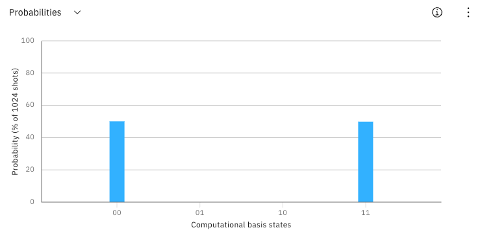
\includegraphics[width=1\textwidth]{images/quantum-information/results_ibm.png}
    \caption{Wahrscheinlichkeitsverteilung - IBM Quantum Learning Platform.}
    \label{fig:meinbild}
\end{figure}


\subsection{Erzeugung eines Bell-Zustands}
Für die Erzeugung eines Bell-Zustands werden zwei grundlegende Quantengatter benötigt: das Hadamard-Gatter und das CNOT-Gatter. Mithilfe dieser beiden Gatter kann eine Quantenschaltung realisiert werden, die jeden einfachen Zwei-Qubit-Eingangszustand (\(\ket{00}, \ket{01}, \ket{10}, \ket{11}\)) in einen Bell-Zustand überführt.

\begin{figure}[h]
  \centering
  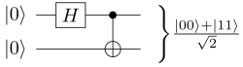
\includegraphics[width=0.4\textwidth]{images/quantum-information/bell_circuit.png}
  \caption{Quantenschaltung zur Erzeugung des Bell-Zustands}
\end{figure}

Die Erzeugung eines Bell-Zustands basiert auf zwei Schritten. Zu Beginn wird eine Superposition erzeugt, anschließend muss die Verschränkung zwischen den Qubits hergestellt werden. Diese Schritte werden nachfolgend erläutert.
\\


\textbf{Schritt 1 – Superposition erzeugen:} \\
Zuerst wird auf das erste Qubit ein Hadamard-Gatter angewendet. Dadurch wird dieses Qubit in eine Superposition überführt:

\[
\frac{1}{\sqrt{2}} (\ket{0} + \ket{1}) \ket{0} = \frac{1}{\sqrt{2}} (\ket{00} + \ket{10})
\]
\\


\textbf{Schritt 2 – Verschränkung herstellen:} \\
Anschließend folgt ein CNOT-Gatter, bei dem das erste Qubit als Kontroll- und das zweite als Zielqubit fungiert. Dieses Gatter invertiert das Zielqubit nur dann, wenn das Kontrollqubit den Zustand \(\ket{1}\) hat. Dadurch entsteht der Zustand:

\[
\frac{1}{\sqrt{2}} (\ket{00} + \ket{11}) = \ket{\Phi^+}
\]


Es resultiert einer der zuvor vorgestellten Bell-Zustände – ein maximal verschränkter Zustand, in dem die Messungen der beiden Qubits perfekt korreliert sind. Wird in einem verschränkten Bell-Zustand das erste Qubit gemessen, so ergibt sich mit gleicher Wahrscheinlichkeit entweder der Zustand \( \ket{0} \) oder \( \ket{1} \). In beiden Fällen legt diese erste Messung sofort auch den Zustand des zweiten Qubits fest: Beobachtet man \( \ket{0} \) am ersten Qubit, ergibt sich insgesamt der Zustand \( \ket{00} \); misst man \( \ket{1} \), resultiert der Zustand \( \ket{11} \). Eine anschließende Messung des zweiten Qubits führt daher zwangsläufig zum gleichen Ergebnis wie beim ersten – entweder beide Qubits liefern 0 oder beide liefern 1. Je nach Eingangs-Zustand und der Reihenfolge der Gatter ergibt sich ein anderer Bell-Zustand. (Vgl. \cite[S.53-54]{homeister_quantum_2022})
\\


Ein anschauliches Beispiel für die Eigenschaften verschränkter Zustände liefert ein Gedankenexperiment mit Alice und Bob. Angenommen die beiden erzeugten gemeinsam entsprechend der vorhergehenden Ausführungen folgenden Bell-Zustand:

\[
\begin{aligned}
\ket{\Phi^+} &= \frac{1}{\sqrt{2}} (\ket{00} + \ket{11}),
\end{aligned}
\]

Alice erhält nun das erste Qubit, Bob das zweite Qubit. Angenommen die beiden bewegen sich, wie nachfolgend abgebildet, anschließend in einem Haus in verschiedene Räume. Solange nun keine Messung erfolgt und die Qubits vor äußeren Einflüssen geschützt sind, bleibt die Verschränkung erhalten. Führen Alice oder Bob eine Messung durch, so ist das Ergebnis: Mit einer Wahrscheinlichkeit von 50\,\% wird $|0\rangle$ gemessen, mit 50\,\% $|1\rangle$. Erst wenn Alice und Bob ihre Ergebnisse miteinander vergleichen, zeigt sich die Besonderheit: Ihre Messergebnisse stimmen stets überein. Es resultiert eine perfekte Korrelation, unabhängig von Raum und Zeit. (Vgl. \cite[S.54]{homeister_quantum_2022})


\begin{figure}[h]
  \centering
  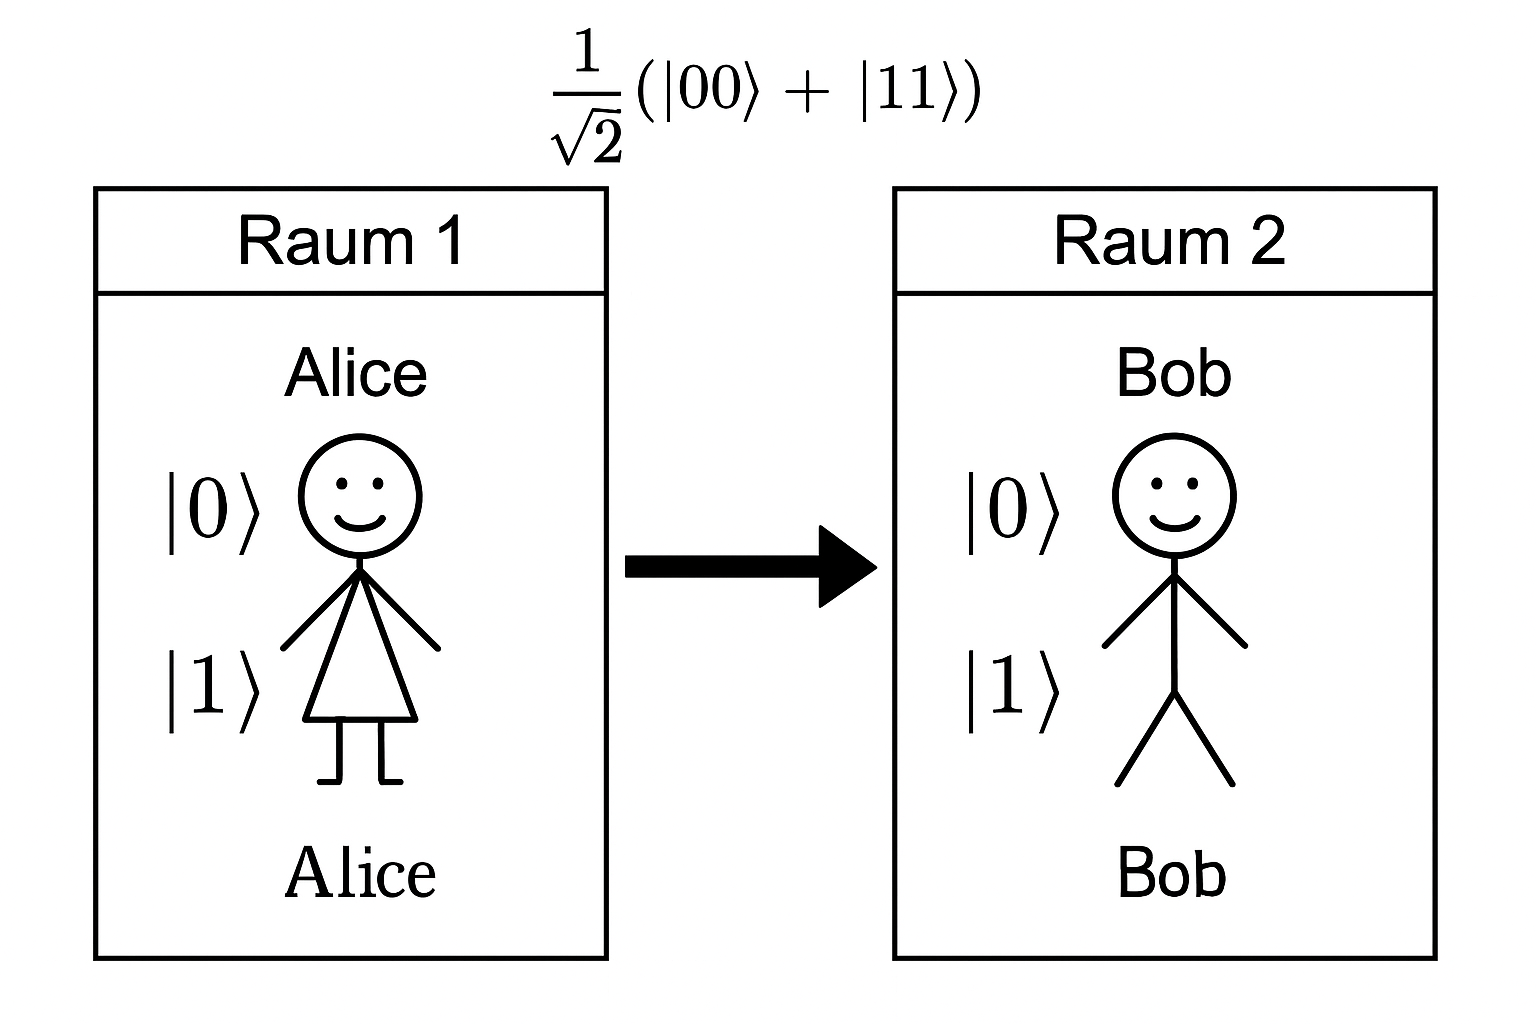
\includegraphics[width=0.5\textwidth]{images/quantum-information/Bell_Alice_Bob.png}
  \caption{Bell-Zustand: Alice und Bob}
\end{figure}



Genau darin zeigt sich der Informationsgehalt eines verschränkten Zustands: Die Information liegt nicht in einem einzelnen Qubit, sondern in ihrer gemeinsamen Beziehung. Diese Simulation macht das abstrakte Konzept der Quantenverschränkung greifbar und bietet einen intuitiven Zugang zu den Grundlagen der Quanteninformation. Es zeigt anschaulich, wie Quantencomputer fundamentale Prinzipien der Quantenmechanik sichtbar und messbar machen. 

\subsection{Bell-Zustand in der Praxis}

Bell-Zustände bilden das Fundament für viele Anwendungsfälle. Ein praktischer Anwendungsfall ist die Quantenkryptographie. Besonders bekannt ist insbesondere das sogenannte E91-Protokoll, welches auf dem Konzept der Quantenverschränkung beruht. Dabei erzeugt eine zentrale Quelle verschränkte Teilchenpaare und schickt je eines an zwei weit entfernte Personen – wie in unserem Beispiel etwa Alice und Bob. Wenn beide ihre Teilchen messen, erhalten sie stets perfekt korrelierte Ergebnisse. Dieser Effekt lässt sich nutzen, um einen gemeinsamen geheimen Schlüssel zu erzeugen. Ein Abhörversuch durch eine dritte Person würde diese Korrelation stören und könnte über einen Bell-Test erkannt werden. So kann mit Hilfe der Quantenmechanik sichergestellt werden, dass keine unbemerkte Informationsweitergabe stattgefunden hat – eine Grundlage für absolut sichere Kommunikation. (Vgl. \cite[S. 3841 f.]{kumar_state---art_2021})
\\


Quantenbasierte Protokolle stehen daher im Zentrum aktueller Forschung zur Quantenkryptographie und wurden bereits in ersten praktischen Experimenten erprobt. Besonders eindrucksvoll ist das Experiment mit dem chinesischen Micius-Satelliten: Er übermittelte verschränkte Photon-Bell-Paare an zwei Bodenstationen, die über eine Entfernung von rund 1200 Kilometern verteilt waren. Die gemessenen Korrelationen verletzten dabei deutlich die Bell-Ungleichung – ein klares Zeichen dafür, dass die beobachteten Effekte nicht durch klassische Physik erklärbar sind, sondern echte Quantenverschränkung vorliegt. Auf dieser Grundlage könnten über Kontinente hinweg geheime Schlüssel erzeugt und die Kommunikation verschlüsselt werden. (Vgl. \cite{ivezic_entanglement_2022})
\\


Ein zweiter praktischer Anwendungsfall des Bell-Zustands findet sich im Quantencomputing, genauer gesagt in der sogenannten Quantenteleportation. Dabei wird der Zustand eines Quantenbits (Qubit) von einem Ort zu einem anderen übertragen, ohne dass das Teilchen selbst physisch bewegt wird. Grundlage hierfür ist ein gemeinsam genutzter Bell-Zustand zwischen Sender (Alice) und Empfänger (Bob), der die nötige Verschränkung bereitstellt. Durch eine spezielle Messung auf Seiten von Alice und die Übermittlung zweier klassischer Bits kann Bob den ursprünglichen Zustand lokal wiederherstellen. (Vgl. \cite{bennett_teleporting_1993})
\\


Im Gegensatz zur Quantenkryptographie, bei der Sicherheit im Vordergrund steht, dient die Quanten-Teleportation der fehlerfreien Übertragung von Quanteninformation. Dies ist eine essenzielle Voraussetzung für die Vernetzung räumlich verteilter Quantencomputer. Sie gilt daher als Schlüsselfunktion zukünftiger Quantencomputer-Netzwerke, etwa im Rahmen eines „Quanteninternets“. (Vgl. \cite{ivezic_entanglement_2022}) Erste praktische Umsetzungen konnten dies bereits demonstrieren: 2017 gelang es ein Qubit über 1.400 km mit dem zuvor bereits erwähnten Satellit Micius erfolgreich zu teleportieren. (Vgl. \cite{ren_ground--satellite_2017})


\section{Zusammenfassung}
In diesem Kapitel wurden zentrale Konzepte der Quanteninformation eingeführt. Ausgangspunkt war das Qubit als quantenmechanisches Pendant zum klassischen Bit. Durch Superposition und komplexe Amplituden besitzt ein Qubit einen kontinuierlichen Zustandsraum, der auf der Bloch-Kugel visualisiert werden kann. In Kombination mit weiteren Qubits eröffnet sich durch Verschränkung ein exponentiell wachsender Zustandsraum, der die Basis für das sogenannte Quantenparallelismus bildet. Mit den Pauli- und Hadamard-Gattern sowie Mehr-Qubit-Gattern wie CNOT und SWAP wurden die grundlegenden Bausteine für Quantenoperationen vorgestellt. Aufbauend darauf wurden die ersten Quantenalgorithmen – insbesondere der Deutsch- und der Deutsch-Josza-Algorithmus – erläutert, die zeigen, wie Quantencomputer bestimmte Probleme effizienter lösen können als klassische Systeme. Darüber hinaus wurde die Bedeutung robuster Fehlerkorrekturmechanismen hervorgehoben, um die hohe Fehleranfälligkeit physikalischer Qubits auszugleichen. Schließlich wurde die Rolle der Quantenverschränkung für Kommunikation und Teleportation aufgezeigt. Anhand der Bell-Zustände wurde demonstriert, wie stark korrelierte Quantenpaare als Grundlage für Quantenkryptographie und verteilte Quantenberechnungen dienen. Insgesamt bietet dieses Kapitel eine Grundlage, um die Funktionsweise und das Potenzial von Quantencomputern zu verstehen und bereitet darauf vor, in den kommenden Kapiteln tiefer in Hardware, Software und konkrete Anwendungen einzutauchen.

\printbibliography
